\documentclass[style=lehigh,orient=landscape]{powerdot}
\pdsetup{
  palette=lehigh,
  logohook=tl,
  logopos={0.005\slidewidth,0.995\slideheight},
  logocmd={
\includegraphics[trim=0 -1 0 0,clip,width=.30\slidewidth,height=.08\slideheight]{lehigh.eps}},
  lf={\color{black}Document Creation with \LaTeX{}},
  %lf={\color{black}\sectiontitle},
  cf={\color{black}HPC Training},
  theslide={\color{black}\arabic{slide}~/~\pageref*{lastslide}}
}
 
\definecolor{pdcolor2}{RGB}{241,231,200}%lucream
\definecolor{pdcolor3}{RGB}{102,55,0}%lubrown
\definecolor{lucyan}{RGB}{0,164,228}
\definecolor{lumagenta}{RGB}{236,81,157}
\definecolor{lugold}{RGB}{255,196,35}
\definecolor{lupurple}{RGB}{125,129,190}

\usepackage{mathtools,amsthm,amssymb,amsfonts}
\usepackage{pifont,tgpagella,marvosym,wasysym}
\usepackage{multicol,multirow}
\usepackage{fancyvrb,listings}
\usepackage{showexpl,enumitem}
\usepackage{graphicx}
\usepackage{rotating}

\renewcommand{\descriptionlabel}[1]%
   {\color{pdcolor2}\textbf{#1}}
\newcommand{\cmark}{\ding{51}}

\lstset{
  language={[LaTeX]TeX},
  %alsolanguage={PGF/TikZ},
  frame=single,
  framesep=\fboxsep,
  framerule=2pt,
%  frameshape={RYRYNYYYY}{yny}{yny}{RYRYNYYYY},
%  fillcolor=\color{pdcolor2},
  rulecolor=\color{pdcolor2},
  xleftmargin=\dimexpr\fboxsep+\fboxrule,
  xrightmargin=\dimexpr\fboxsep+\fboxrule,
  breaklines=true,
  basicstyle=\scriptsize\tt,
  keywordstyle=\color{cyan}\sf,
  morekeywords={part,chapter,subsection,subsubsection,paragraph,subparagraph},
  identifierstyle=\color{magenta},
  commentstyle=\color{red},
  backgroundcolor=\color{pdcolor3},
  tabsize=2,
  columns=flexible,
  escapeinside={\%*}{*)},
}

\title{Document Creation with \LaTeX{}}
\author{Alexander B. Pacheco}

\date{LTS Research Computing}

\begin{document}
\maketitle
\begin{wideslide}[toc=,bm=]{Overview}
  \tableofcontents[content=sections]
\end{wideslide}
\scriptsize

\section[slide=false]{Introduction}
\begin{wideslide}[toc=,bm=]{Overview}
  \tableofcontents[content=currentsection,type=0]
\end{wideslide}
%	\section[tocsection=true,slide=true]{Introduction}
\begin{wideslide}[bm={What is \TeX{} \& \LaTeX?}]{What is \TeX{}?}
  \begin{itemize}
  \item \TeX{} is a low-level markup and programming language created by Donald Knuth to typeset documents attractively and consistently.
  \item \TeX{} is a programming language in the sense that it supports the if-else construct: you can make calculations with it (that are performed while compiling the document), etc., but you would find it very hard to do anything else but typesetting with it.
  \item The fine control \TeX{} offers over document structure and formatting makes it a powerful and formidable tool.
  \item \TeX{} is renowned for being extremely stable, for running on many different kinds of computers, and for being virtually bug free.
  \item \TeX\, is a popular means by which to typeset complex mathematical formulae; it has been noted as one of the most sophisticated digital typographical systems in the world.
  \item Programming in \TeX{} generally progresses along a very gradual learning curve, requiring a significant investment of time to build custom macros for text formatting.
  \item Document preparation systems based on \TeX{}, consisting of collections of pre-built macros, exist making it easier for the user to create documents without the need to learn the \TeX{} language.
  \end{itemize}
\end{wideslide}	

\begin{wideslide}[bm={What is \LaTeX{}?}]{What is \LaTeX{}?}
  \begin{itemize}
  \item \LaTeX{} is a macro package based on \TeX{} created by Leslie Lamport.
  \item Its purpose is to simplify \TeX{} typesetting, especially for documents containing mathematical formulae.
  \item Popular in academia, especially in mathematics, computer science, economics, engineering, physics, statistics, and quantitative psychology.
  \item Many of the academic publishing houses such as American Institute of Physics, Elsevier, etc provide templates to prepare manuscripts in \LaTeX{}.
  \item Since \LaTeX{} comprises a group of \TeX{} commands, \LaTeX{} document processing is essentially programming.
  \item Using \LaTeX{} to create documents is a WYSIWYM (What You See Is What You Mean) approach rather than 
  \item[] WYSIWYG (What You See Is What You Get) approach of Microsoft Word and Libre Office.
  \item In \LaTeX{}, you create a text file in \LaTeX{} markup, which then needs to be compiled to produce the final document, most commonly is postscript (ps) or portable document format (pdf).
  \item The final document can be viewed uniformly on any Operating System using any version of the document viewer.
  \end{itemize}
\end{wideslide}

\begin{wideslide}[bm={Advantages of \LaTeX{}?}]{Advantages of \LaTeX{}?}
  \begin{itemize}
  \item Document sources can be read with any text editor.
  \item You can concentrate purely on the structure and contents of the document, not get caught up with superficial layout issues.
  \item You don't need to manually adjust fonts, text sizes, line heights, or text flow for readability, as \LaTeX{} takes care of them automatically.
  \item In \LaTeX{} the document structure is visible to the user, and can be easily copied to another document.
  \item The layout, fonts, tables and so on are consistent throughout the document.
  \item Mathematical formulae can be easily typeset.
  \item Indexes, footnotes, citations and references are generated easily.
  \item Since the document source is plain text, tables, figures, equations, etc. can be generated programmatically with any language.
  \item You are forced to structure your documents correctly.
  \end{itemize}
\end{wideslide}

\begin{wideslide}[bm={Disadvantages of \LaTeX{}?}]{Disadvantages of \LaTeX{}?}
  \begin{itemize}
  \item \LaTeX{} is WYSIWYM and not WYSIWYG approach
  \item[] i.e. you can't see what the final version will look like while typing.
  \item You need to know the necessary commands for the markup language.
  \item[] i.e. there is no drop-down menu to create the document content such as equations, tables, inserting figures etc, you need to know how to enter those in a text editor.
  \item It can sometimes be difficult to obtain a certain look for the document.
  \end{itemize}
\end{wideslide}

\begin{wideslide}[toc=,bm={Terms regarding \TeX{}}]{Document Preparation Systems}
  \begin{itemize}
  \item A document preparation system such as \LaTeX{} is the combination of the \TeX{} language and the macros.
    \begin{description}
    \item[LaTeX]: designed by Leslie Lamport, it is actually a set of macros for TeX. It aims at taking care of the formatting process.
    \item[ConTEXT]: has a very consistent and easy syntax and support for pdfTeX, XeTeX and LuaTeX engines.
    \item[TeX]: The original language designed by Donald Knuth
      %\item \XeTeX{} \AMSLaTeX{} \BibTeX{} \WinEdt{} \LyX{} \ConTeXt{} \MikTeX{}
    \end{description}
  \item Engines
    %  \begin{ablock}{Engines}
    \begin{itemize}
    \item An engine is an executable that can turn your source code into a printable output format. 
    \item The engine by itself only handles the syntax, it also needs to load fonts and macros to fully understand the source code and generate output properly. 
    \item The engine will determine what kind of source code it can read, and what format it can output (usually DVI or PDF).
    \end{itemize}
    \begin{description}
    \item[{pdftex,pdflatex}]: PDF compilers
    \item[{tex,latex}]: DVI compilers
    \item[{luatex,lualatex}]: A TeX engine with Lua scripting engine embedded
    \end{description}
    %  \end{ablock}
  \end{itemize}
\end{wideslide}

\begin{wideslide}[toc=]{Installing \LaTeX}
  \begin{itemize}
%  \begin{bblock}{Distributions}
    \item Distributions
      \begin{itemize}
      \item TeX distributions are collections of packages and programs (compilers, fonts, and macro packages) that enable you to typeset without having to manually fetch files and configure things.
      \end{itemize}
      \begin{description}
      \item[{TeX Live}]: A cross platform TeX distribution \url{http://www.tug.org/texlive}
      \item[{MacTeX}]: A TeX Live based distribution targeting Mac OS X \url{http://www.tug.org/mactex}
      \item[{MikTeX}]: A TeX distribution for Windows \url{http://www.miktex.org}
      \end{description}
%  \end{bblock}
    \item Installation:
      \begin{enumerate}
      \item On Mac OSX, download the zip file and follow the instructions
      \item On Windows, MikTeX has an easy installer that takes care of setting up the environment and downloading core packages.
      \item On Linux, use the package manager (apt-get, yum, zypper etc) to download and install texlive and other additional packages. 
      \item[] texlive should be present in main repositories. If not, your distribution web-site will have additional information.
      \end{enumerate}
  \end{itemize}
\end{wideslide}

%\begin{wideslide}[toc=]{Distributions}
%  \begin{itemize}
%  \item TeX distributions are collections of packages and programs (compilers, fonts, and macro packages) that enable you to typeset without having to manually fetch files and configure things.
%  \end{itemize}
%  \begin{description}
%  \item[{TeX Live}]: A cross platform TeX distribution \url{http://www.tug.org/texlive}
%  \item[{MacTeX}]: A TeX Live based distribution targeting Mac OS X \url{http://www.tug.org/mactex}
%  \item[{MikTeX}]: A TeX distribution for Windows \url{http://www.miktex.org}
%  \end{description}
%\end{wideslide}

\begin{wideslide}[toc=]{Which Editors to use to typeset documents?}
  \begin{itemize}
  \item TeX and LaTeX source documents (as well as related files) are all text files, and can be opened and modified in almost any text editor.
  \item You should use a text editor (e.g. Notepad), not a word processor (Word, OpenOffice).
  \end{itemize}
  \vspace{-0.5cm}
    \begin{center}
      \begin{tabular}{|c|c|ccc|}
        \hline
        Type & Editor       & Windows & Mac OS X & Linux  \\
        \hline
        \multirow{5}{*}{Text Editor} & Vim          & \cmark  & \cmark   & \cmark \\
                                     & Emacs        & \cmark  & \cmark   & \cmark \\
                                     & gedit        &         &          & \cmark \\
                                     & kate         &         &          & \cmark \\
                                     & Notepad      & \cmark  &          &        \\
        \hline
        \multirow{3}{*}{WYSIWYG Editor} & LyX          & \cmark  & \cmark   & \cmark \\
                                        & Bakoma TeX   & \cmark  & \cmark   & \cmark \\
                                        & Gummi        & \cmark  &          & \cmark \\
        \hline
        \multirow{8}{*}{\LaTeX{} Editor} & TeXmaker     & \cmark  & \cmark   & \cmark \\
                                         & TeXstudio    & \cmark  & \cmark   & \cmark \\
                                         & TeXworks     & \cmark  & \cmark   & \cmark \\
                                         & Kile         &         &          & \cmark \\
                                         & TeXshop      &         & \cmark   &        \\
                                         & TeXnicle     &         & \cmark   &        \\
                                         & WinEdt       & \cmark  &          &        \\
                                         & TeXnicCenter & \cmark  &          &        \\
        \hline
        \multirow{3}{*}{Web Based}       & Share\LaTeX{} & \multicolumn{3}{c|}{\url{https://www.sharelatex.com}}\\
                                         & Overleaf      & \multicolumn{3}{c|}{\url{https://www.overleaf.com}}\\
                                         & Authorea      & \multicolumn{3}{c|}{\url{https://authorea.com}}\\
        \hline
        \end{tabular}
    \end{center}
%    \begin{enumerate}
%    \item Document sources can be read and edited with any text editor such as
%    \item[\normalsize{\color{pdcolor2}\ding{229}}] vi/vim, emacs, gedit, kate, kwrite, Notepad. Word and OpenOffice are not text editors.
%    \item There are other editors some with WYSIWYG-like features that take care of compiling the LaTeX source and updating it constantly to view changes to document almost in real time.
%    \item[\normalsize{\color{pdcolor2}\ding{229}}] BaKoMa TeX (Windows \& Mac OS), Gummi (Linux \& Windows), LyX
%    \item Dedicated \LaTeX{} editors that have auto-completion of commands, spell and error checking and handy macros.
%    \item[\normalsize{\color{pdcolor2}\ding{229}}] TeXmaker, TeXstudio, TeXworks, Kile (Linux), WinEdt and TeXnicCenter (Windows).
%    \end{enumerate}
\end{wideslide}

\section[slide=false]{\LaTeX{} Basics}
\begin{wideslide}[toc=,bm=]{Overview}
  \tableofcontents[content=currentsection,type=0]
\end{wideslide}

\begin{wideslide}[bm={Syntax},method=file]{Syntax}
  \begin{itemize}
  \item LaTeX uses a markup language in order to describe document structure and presentation.
  \item LaTeX converts your source text, combined with the markup, into a high quality document.
  \item For the purpose of analogy, web pages work in a similar way: the HTML is used to describe the document, but it is your browser that presents it in its full glory - with different colors, fonts, sizes, etc.
  \item "Whitespace" characters such as space or tab are treated uniformly as "space" by LaTeX.
  \item Several consecutive whitespace characters are treated as one "space".
  \end{itemize}	
%  \begin{lstlisting}
%Several consecutive whitespace characters such as          are treated as one space
%  \end{lstlisting}
  \begin{LTXexample}[numbers=none,showspaces=true,pos=b]
Several consecutive whitespace characters such as          are treated as one space
  \end{LTXexample}
\end{wideslide}

\begin{wideslide}[bm={Reserved Characters},method=direct]{Reserved Characters}
  \begin{itemize}
  \item LaTeX has special characters or symbols that either have a special meaning or are bit available in all fonts.
  \item If you enter them directly in your text, they will normally not print.
  \item To print these symbols, you need to be escape with a \textbackslash{} except \textbackslash{} itself since \textbackslash\textbackslash{} is reserved for line break.
  \end{itemize}
  \begin{center}
    \begin{tabular}{|ccc|}
      \hline
      Symbol & Command & Usage\\
      \hline
      \# & \verb|\#| & reference arguments \\
      \% & \verb|\%| & Comment\\
      \$ & \verb|\$| & Math Mode\\
      \^{} & \verb|\^| & Superscript\\
      \_ & \verb|\_| & Subscript\\
      \& & \verb|\&| & Alignment\\
      \{ \} & \verb|\{ \}| & wrap arguments\\
%      \} & \verb|\}| & end wrap arguments\\
      \~{} & \verb|\~| & produce non-breakable space \\
      \textbackslash & \verb|\textbackslash| & escape character\\
      \textbackslash\textbackslash & \verb|\\| & line break\\
      \hline
    \end{tabular}
  \end{center}
\end{wideslide}

\begin{wideslide}[bm={Environments},method=direct]{Environments}
  \begin{itemize}
  \item Environments in LaTeX have a role that is quite similar to commands, but they usually have effect on a wider part of the document. 
  \item Their syntax is:
    \begin{lstlisting}
\begin{environmentname}
text to be influenced
\end{environmentname}
    \end{lstlisting}
  \item Between the \lstinline|\begin| and the \lstinline|\end| you can put other commands and nested environments. 
  \item The internal mechanism of environments defines a group, which makes its usage safe (no influence on the other parts of the document).
  \item In general, environments can accept arguments as well, but this feature is not commonly used and so it will be discussed in more advanced parts of the document.
  \item Anything in LaTeX can be expressed in terms of commands and environments.
  \end{itemize}	
\end{wideslide}

\begin{wideslide}[bm={Groups},method=direct]{Groups}
  \begin{itemize}
  \item A group is basically defined by a pair of braces.
  \item The range of commands put between braces is limited to them.
  \item Example
  \end{itemize}	
  \begin{LTXexample}[numbers=none,pos=b]
{\bf This is in bold}\\
{\em This is in italics}
This is normal text
  \end{LTXexample}
\end{wideslide}

\begin{wideslide}[bm={Commands},method=direct]{Commands}
  \begin{itemize}
  \item LaTeX commands are case sensitive, and take one of the following two formats:
    \begin{itemize}
    \item They start with a backslash \textbackslash and then have a name consisting of letters only. Command names are terminated by a space, a number or any other "non-letter".
    \item They consist of a backslash \textbackslash and exactly one non-letter.
    \end{itemize}
  \item Some commands need an argument, which has to be given between curly braces \{ \} after the command name. 
  \item Some commands support optional parameters, which are added after the command name in square brackets [ ]. 
  \item The general syntax is:
    \lstinline|\commandname[option1,option2,...]{argument1}{argument2}...|
  \item Most standard LaTeX commands have a switch equivalent. 
  \item Switches have no arguments but apply on the rest of the scope, i.e. the current group or environment. 
  \item A switch should (almost) never be called outside of any scope, otherwise it will apply on the rest of the document.
    \begin{LTXexample}[numbers=none,pos=r]
{\bf This is in bold}\\
\em This is in italics
This is normal text
  \end{LTXexample}
  \end{itemize}	
\end{wideslide}

\begin{wideslide}[bm={Comments},method=direct]{Comments}
  \begin{itemize}
  \item When LaTeX encounters a \% character while processing an input file, it ignores the rest of the current line, the line break, and all whitespace at the beginning of the next line.
  \item This can be used to write notes into the input file, which will not show up in the printed version.
    \begin{LTXexample}[numbers=none,pos=b,showspaces=true]
This is an % stupid
% Better: instructive <----
example: Supercal%
            ifragilist%
icexpialidocious
    \end{LTXexample}
  \item Note that the \% character can be used to split long input lines that do not allow whitespace or line breaks, as with Supercalifragilisticexpialidocious above.
  \item The core LaTeX language does not have a predefined syntax for commenting out regions spanning multiple lines.
  \end{itemize}	
\end{wideslide}
z
\begin{wideslide}[method=direct]{Type Fonts}
  \begin{itemize}
  \item The actual letters and symbols (collectively called type) that LaTeX produces are characterized by their style and size.
  \item A type style is specified by family, series and shape.
  \item Default font type is roman family, medium series and upright shape.
  \end{itemize}
  \begin{center}
    \begin{tabular}{|c|c|c|c|c|}
      \cline{2-5}
      \multicolumn{1}{c}{} & \multicolumn{1}{|c|}{\textsc{style}} & \multicolumn{1}{|c|}{\textsc{command}} & \multicolumn{2}{|c|}{\textsc{Alternate declaration}}\\
      \hline
      \multirow{3}{*}{\textsc{Family}} & \textrm{roman} & \lstinline|\textrm{roman}| & \lstinline|{\rmfamily roman}| & \lstinline|{\rm roman}|\\
      & \textsf{sans serif} & \lstinline|\textsf{sans serif}| & \lstinline|{\sffamily sans serif}| & \lstinline|{\sf sans serif}|\\
      & \texttt{typewriter} & \lstinline|\texttt{typewriter}| & \lstinline|{\ttfamily typewriter}| & \lstinline|{\tt typewriter}|\\
      \hline
      \multirow{2}{*}{\textsc{series}} & \textmd{medium} & \lstinline|\textmd{medium}| & \lstinline|{\mdseries medium}| & \\
      & \textbf{boldface} & \lstinline|\textbf{boldface}| & \lstinline|{\bfseries boldface}| & \lstinline|{\bf boldface}|\\
      \hline
      \multirow{4}{*}{\textsc{shape}} & \textup{upright} & \lstinline|\textup{upright}| & \lstinline|{\upshape upright}| & \\
      & \textit{italics} & \lstinline|\textit{italics}| & \lstinline|{\itshape italics}| & \lstinline|{\it italics}|\\
      & \textsl{slanted} & \lstinline|\textsl{slanted}| & \lstinline|{\slshape slanted}| & \lstinline|{\sl slanted}|\\
      & \textsc{small cap} & \lstinline|\textsc{small cap}| & \lstinline|{\scshape small caps}| & \lstinline|{\sc small caps}|\\
      \hline
    \end{tabular}
  \end{center}
\end{wideslide}

\begin{wideslide}[method=direct]{Type Size}
  \begin{itemize}
    \item Type size is traditional measured in (printer) points.
    \item The default type produced by LaTeX documents is 10pt size.
    \item To change the type size, LaTeX has ten declarations available
  \end{itemize}
  \begin{center}
    \begin{tabular}{|c|c|c|c|}
      \hline
      {\tiny size} & \lstinline|{\tiny size}| & {\large size}  & \lstinline|{\large size}| \\
      {\scriptsize size} & \lstinline|{\scriptsize size}| & {\Large size} & \lstinline|{\Large size}| \\
      {\footnotesize size} & \lstinline|{\footnotesize size}| & {\LARGE size}  & \lstinline|{\LARGE size}| \\
      {\small size} & \lstinline|{\small size}| & {\huge size} & \lstinline|{\huge size}| \\
      {\normalsize size} & \lstinline|{\normalsize size}| & {\Huge size} & \lstinline|{\Huge size}| \\
      \hline
    \end{tabular}
  \end{center}
\end{wideslide}

\begin{wideslide}[bm={My First \LaTeX{} Document},method=direct]{My First \LaTeX{} Document}
  \begin{itemize}
  \item Using your favorite text editor, create a file \texttt{hello.tex} that contains the following lines.
  \end{itemize}	
  \begin{lstlisting}
    %My First LaTeX Document
    \documentclass{article}
    \begin{document}
    Hello World!
    \end{document}
  \end{lstlisting}
  \begin{itemize}
  \item The first line is a comment. All comments begin with \% symbol.
  \item The second line tells LaTeX to use the article document class.
  \item The \lstinline|\begin{document}| command begins the actual document, while
  \item \lstinline|\end{document}| command ends the document.
  \item The document content goes within \lstinline|\begin{document}| and \lstinline|\end{document}| commands.
  \end{itemize}
\end{wideslide}

\begin{wideslide}[bm={Compile \LaTeX{} Document},method=direct]{Compiling \LaTeX{} Document}
  \begin{itemize}
  \item Run one of the following two sets of commands from the command prompt
    \begin{enumerate}
    \item \texttt{\color{pdcolor2}latex hello}
    \item \texttt{\color{pdcolor2}dvips hello} (If you can view postscript files)
    \item \texttt{\color{pdcolor2}dvipdf hello}
    \end{enumerate}
  \item[\textbf{\color{pdcolor2}OR}]
    \begin{enumerate}
    \item \texttt{\color{pdcolor2}pdflatex hello}
    \end{enumerate}
  \item Open the pdf file created i.e. \texttt{\color{pdcolor2}hello.pdf}
  \item If your computer has a DVI or postscript viewer, you can view the \texttt{\color{pdcolor2}hello.dvi} or \texttt{\color{pdcolor2}hello.ps} files.
  \end{itemize}
\end{wideslide}

\begin{wideslide}[bm={Ancillary Files}]{Ancillary Files}
  \begin{itemize}
    \item LaTeX compilation creates a bunch of files with various extensions to store temporary data to use for next compilation
    \item[\color{pdcolor2}.aux]: A file that transports information from one compiler run to the next. Among other things, the .aux file is used to store information associated with cross-references.
    \item[\color{pdcolor2}.log]: Gives a detailed account of what happened during the last compiler run.
    \item[\color{pdcolor2}.toc]: Stores all your section headers. It gets read in for the next compiler run and is used to produce the table of contents.
    \item[\color{pdcolor2}.lof]: This is like .toc but for the list of figures.
    \item[\color{pdcolor2}.lot]: And again the same for the list of tables.
    \item[\color{pdcolor2}.bbl]: Bibliography file output by BiBTeX and used by LaTeX
    \item[\color{pdcolor2}.blg]: BiBTeX log file. (errors are logged here)
    \item[\color{pdcolor2}.dvi]: Device Independent File. This is the main result of a LaTeX compile run with latex. You can look at its content with a DVI previewer program or you can send it to a printer with dvips or a similar application.
  \end{itemize}
\end{wideslide}

\begin{emptyslide}[toc=,bm=]{}
\centering
\vspace{\stretch{1}}

\includegraphics[height=0.9\slideheight]{./hello.ps}
\vspace{\stretch{1}}
\end{emptyslide}

\section[slide=false]{Document Structure}
\begin{wideslide}[toc=,bm=]{Overview}
  \tableofcontents[content=currentsection,type=0]
\end{wideslide}

\begin{wideslide}[toc=,method=direct]{\LaTeX{} File Structure}
  \begin{itemize}
  \item When LaTeX processes an input file, it expects it to follow a certain structure.
  \item Every LaTeX input file must contain the commands,
    \begin{lstlisting}
\documentclass{...}

\begin{document}
...
\end{document}
    \end{lstlisting}
  \item The area between \lstinline|\documentclass{...}| and \lstinline|\begin{document}| is called the {\bf Preamble}.
  \item The document content goes between the \lstinline|\begin{document}| and \lstinline|\end{document}| commands,
    \begin{lstlisting}
\begin{document}
   ...
\end{document}
    \end{lstlisting}
%  \item The reason for marking off the beginning of your text is that LaTeX allows you to insert extra setup specifications before it.
%  \item The reason for marking off the end of your text is to provide a place for LaTeX to be programmed to do extra stuff automatically at the end of the document, like making an index.
  \end{itemize}
\end{wideslide}

\begin{wideslide}{Preamble}
  \begin{itemize}
  \item The Preamble is anything that comes before the main document.
  \item It is used for
    \begin{itemize}
    \item Defining the type of document.
    \item Defining the top matter i.e. title, author, etc.
    \item Applying global formatting including changing page layout from the default.
    \item Including packages to add functionality.
    \end{itemize}
  \end{itemize}
\end{wideslide}

\begin{wideslide}[bm={Document Types},method=direct]{Document Types}
  \begin{itemize}
  \item The first uncommented line of the LaTeX document needs to describe the type of document that you are creating using
  \item[] \lstinline|\documentclass[options]{documenttype}|
  \item LaTeX can be used to create documents of various types
    \begin{enumerate}
    \item article
    \item report
    \item book
    \item letter
    \item beamer\footnote{\tiny For Tutorial, visit \url{http://www.hpc.lsu.edu/training/archive/tutorial.php}}, {\color{pdcolor2}powerdot}\footnote{\tiny{\sc this presentation}, style file included in downloads}, {\color{red}prosper or seminar\footnote{\tiny Not popular anymore, use beamer or powerdot}} for Presentations
    \end{enumerate}
  \item The difference between article, report and book is in the document structure and presentation:
  \item In article type, there is no chapter and the title page and document content can appear on the first page.
  \item In report and book, the title page is the first page and document content begins on the second page onwards.
  \item In article and report, there is an abstract environment to write the abstract of the article or report that you are writing.
  \vspace{0.2cm}
  \end{itemize}
\end{wideslide}

\begin{wideslide}[bm={documentclass options}]{documentclass options}
  \begin{itemize}[][itemsep=1pt,parsep=1pt]
  \item The options to documentclass are used to define a predetermined structure for the document.
  \item The most commonly used options are defining
    \begin{itemize}[][itemsep=1pt,parsep=1pt]
    \item font size: 10pt (default), 11pt or 12pt
    \item paper size: letterpaper (default), legalpaper, executivepaper, a4paper, a5paper or b5paper
    \item orientation: portrait (default) or landscape
    \item page format: onecolumn (default) or twocolumn
    \end{itemize}
  \item Options that depend on document type
    \begin{itemize}[][itemsep=1pt,parsep=1pt]
    \item Where to print page numbers for book, report and article
      \begin{itemize}[][itemsep=1pt,parsep=1pt]
      \item[{\bfseries\color{pdcolor2}oneside}] page numbers are printed the same on even and odd pages, default for article \& report
      \item[{\bfseries\color{pdcolor2}twoside}] page number appears on the right side for odd pages and on the left for even pages, default for book
      \end{itemize}
    \item Where new chapters begin in the book and report class
      \begin{itemize}[][itemsep=1pt,parsep=1pt]
      \item[{\bfseries\color{pdcolor2}openright}] chapters start on the right hand insert blank page if necessary i.e. odd numbered page
      \item[{\bfseries\color{pdcolor2}openany}] chapters always start on the next page
      \end{itemize}
    \item Where the title appears
      \begin{itemize}[][itemsep=1pt,parsep=1pt]
      \item In book and report classes, the title appears on the first page separate from the document content
      \item In article class, the title appears on the first page followed by the document content
      \item Use {\bfseries\color{pdcolor2}titlepage} and {\bfseries\color{pdcolor2}notitlepage} to override this standard behavior.
      \end{itemize}
    \end{itemize}
  \end{itemize}
\end{wideslide}

\begin{wideslide}[toc=,bm=,method=direct]{documentclass options}
  \begin{itemize}
    \item Other options commonly used
      \begin{description}
        \item[{leqno}]: display equation numbers on the left rather than the default right
        \item[{fleqn}]: displayed formulas are flushed left instead of default centered
        \item[{draft}]: mark lines that are too wide with a thick black bar
        \item[{final}]: default, do not mark lines that are too wide.
      \end{description}
    \item Add some options to documentclass to create your second document.
  \end{itemize}
  \begin{lstlisting}
\documentclass[12pt,twocolumn,fleqn]{article}
  \end{lstlisting}
\end{wideslide}

\begin{wideslide}[method=direct]{Creating a Title Page}
  \begin{itemize}[][itemsep=1pt,parsep=1pt]
  \item To create a title page LaTeX has three commands.
    \begin{itemize}[][itemsep=1pt,parsep=1pt]
      \item \lstinline|\title{Title}| where Title is the title of your article, book or report.
      \item \lstinline|\author{FirstName LastName}|, if there are multiple authors, list them all delimited by a comma (,) or and.
      \item \lstinline|\date{\today}| to set the date when the article was created i.e. today
      \item[] If the date required is different from today, add the date that you need as in \lstinline|\date{Feb. 29, 2016}|
    \end{itemize}
    \item If you are publishing a journal article, please see their LaTeX templates and style files. Most of their style and class files  define additional commands such as \lstinline|\affiliation{...}|, \lstinline|\institution{...}|, etc.
    \item To create the actual page, you need to add \lstinline|\maketitle| in your document i.e. after the \lstinline|\begin{document}| command.
    \item The \lstinline|\maketitle| is almost always the first line of your document content.
  \end{itemize}
      \begin{lstlisting}
\documentclass[12pt,twocolumn,fleqn]{article}
\title{Simple \LaTeX{} Document}
\author{Alex Pacheco, Bhupender Thakur, Feng Chen and Le Yan}
\date{\today}
\begin{document}
\maketitle
\end{document}
      \end{lstlisting}
\end{wideslide}

\begin{wideslide}[bm={Document Structure},method=direct]{Structuring a \LaTeX{} Document}
  \begin{itemize}
    %  \item A LaTeX document consists of two parts
    %    \begin{enumerate}
    %    \item Preamble
    %    \item Main Document
    %      \begin{itemize}
  \item Document Content i.e. everything between the \lstinline|\begin{document}| and \lstinline|\end{document}| is partitioned into
  \end{itemize}
  \begin{center}
    \begin{tabular}{llcl}
      \hline
      Section & Command & Level & Comment\\
      \hline
      part & \lstinline|\part{title}| & -1 & not in letters \\
      chapter & \lstinline|\chapter{title}| & 0 & only in book and report \\
      section & \lstinline|\section{title}| & 1 & not in letters \\
      subsection & \lstinline|\subsection{title}| & 2 & not in letters \\
      subsubsection & \lstinline|\subsubsection{title}| & 3 & not in letters \\
      paragraph & \lstinline|\paragraph{title (optional)}| & 4 & not in letters \\
      subparagraph & \lstinline|\subparagraph{title (optional)}| & 5 & not in letters \\
      \hline
    \end{tabular}
  \end{center}
  %    \begin{itemize}
  %    \item abstract (article and report only)
  %    \item part (-1)
  %    \item chapter (0)
  %    \item section (1)
  %    \item subsection (2)
  %    \item subsubsection (3)
  %    \item paragraph (4)
  %    \item subparagraph (5)
  %    \item appendix
  %    \item Bibliography if applicable
  %    \end{itemize}
  \begin{itemize}
  \item LaTeX provides 7 levels of depth for defining sections. The depth levels for the various commands are listed in column three in the above table. 
  \item The depth level of a section affects whether that section appears in the table of content or not. This can however be changed as we will see in the next few slides.
  \item Since LaTeX is used very often for writing scientific articles and reports, there are environments defined to create Abstract, Appendices and Bibliographies.
  \end{itemize}
  %    \end{enumerate}
  %  \end{itemize}
\end{wideslide}

\begin{wideslide}[method=direct]{Section Numbering}
  \begin{itemize}
  \item Numbering of the sections is performed automatically by LaTeX.
  \item Parts get roman numerals (Part I, Part II, etc.); 
  \item chapters and sections get decimal numbering, and 
  \item appendices (which are just a special case of chapters, and share the same structure) are lettered (A, B, C, etc.).
%  \item In book and report, the numbering style by default is chapter \#.section \#.subsection \#.subsubsection \# as in 1.2.1.3
%  \item In article, the numbering style is section \#.subsection \#.subsubsection \# as in 1.2.1
%  \item Appendices are chapters in book and report and sections in article. Numbering is same as above except the first character is a letter and not a number i.e. A.2.1.3 and A.2.1 for the above two examples respectively.
  \item You can change the depth to which section numbering occurs, so you can turn it off selectively. By default it is set to 2.
  \item To change the depth level, use the \lstinline|\setcounter| command.
  \item For example, to change depth to only include chapters: \lstinline|\setcounter{secnumdepth}{1}|
  \item You can change the numbering mechanism of the sectioning commands as well as lists, captions, equations, tables, figures etc. We'll discuss more about this when we get to user defined commands.
  \end{itemize}
\end{wideslide}

\begin{wideslide}[toc=,method=direct]{Abstract Environment}
  \begin{itemize}
  \item As most research papers have an abstract, there are predefined commands for telling LaTeX which part of the content makes up the abstract. 
    \begin{itemize}
    \item This should appear in its logical order, therefore, after the top matter, but before the main sections of the body. 
    \item {\color{pdcolor2}\emph{This command is available for the document classes article and report, but not book.}}
    \item In document class report, the abstract appears on a separate page without a page number.
    \item In document class article, the abstract comes after the title heading on the first page.
    \end{itemize}
  \end{itemize}
  \begin{LTXexample}[numbers=none,pos=b]
\begin{abstract}
In this article we discuss how to create simple LaTeX documents. Topics include structuring a document, list environment, inserting equations and figures, creating tables and more.
\end{abstract}
  \end{LTXexample}
\end{wideslide}

\begin{wideslide}[toc=,method=direct]{Sectioning}
  \begin{itemize}
    \item The following commands are available for producing automatic, sequential sectioning
    \item[] \lstinline|\part|, \lstinline|\chapter|, \lstinline|\section|, \lstinline|\subsection|, \lstinline|\subsubsection|, \lstinline|\paragraph|, \lstinline|\subparagraph|
    \item Except for \lstinline|\part|, these commands form a sectioning hierarchy.
    \item In document class report and book, the highest sectioning level is \lstinline|\chapter| while in article class, it is \lstinline|\section|.
    \item The chapters are divided into sections using the \lstinline|\section| command, which is further divided into subsections using the \lstinline|\subsection| command and so on.
    \item The syntax for these commands is \lstinline|\command[short title]{title}| or \lstinline|\command*{title}|
    \item In the first form, the section is given the next number in the sequence which is then printed together with a heading using the text "title".
    \item The text "short title" becomes the entry in the table of contents and page head. If "short title" is omitted, then the "title" is used.
    \item In the second form (with *), no section number is printed and no entry is created in the table of contents.
    \item The highest sectioning command is given a single number (1,2,$\cdots$), the second highest command then creates a double number (1.1, 2.3, $\cdots$) and so on.
    \item The paragraph and subparagraph commands are not numbered.
    \item For each sectioning command, there is an internal counter that is incremented by one every time that command is called and reset to zero on every call to a higher sectioning command.
  \end{itemize}
\end{wideslide}

\begin{wideslide}[toc=,bm=,method=direct]{Sectioning (contd)}
  \vspace{-0.4cm}
  \begin{itemize}
  \item The sectioning command, \lstinline|\part| is a special case and does not affect the numbering of other sectioning commands.
  \item The \lstinline|\part| are usually numbered with Uppercase Roman Numerals as in Part I, Part IV, etc.
  \item The \lstinline|\part| is used to divide your document into multiple parts which can be independent of each other.
  \end{itemize}
  \vspace{-0.25cm}
  \twocolumn%[colsep=10pt,lcolwidth=0.4\slidewidth,rcolwidth=0.5\textwidth]
            {\lstinputlisting[basicstyle=\fontsize{4}{5}\selectfont\tt]{./part.tex}}
            {\lstinputlisting[basicstyle=\fontsize{4}{5}\selectfont\tt]{./partreport.tex}}
    
\end{wideslide}

\begin{emptyslide}[toc=,bm=]{}
  \includegraphics[height=\slidewidth,angle=90]{./apart.ps}
\end{emptyslide}

\begin{emptyslide}[toc=,bm=]{}
  \includegraphics[height=\slidewidth,angle=90]{./apartreport.ps}
\end{emptyslide}

\begin{wideslide}[method=direct]{Appendix}
  \begin{itemize}
    \item An appendix is introduced with the declaration \lstinline|\appendix|
    \item The \lstinline|\appendix| resets the section counter in article and chapter counter in book and report.
    \item The numbering for the sectioning commands is also changed from numerals to capital letters, A, B, $\cdots$
    \item The word "Chapter" is replaced by "Appendix" so that subsequent chapter headings are preceded by "Appendix A", "Appendix B", etc.
    \item The numbering of lower sectioning commands contain the letter in place of chapter number, for e.g. A.2.1
  \end{itemize}
  \begin{lstlisting}
\appendix
\section{My First Appendix}
...
\subsection{Subsection in My First Appendix}
...
  \end{lstlisting}
\end{wideslide}

\begin{wideslide}[method=direct]{Cross Referencing}
  \begin{itemize}
  \item Since the various sectioning commands are numbered automatically, the chapter, section, etc numbers may not be known at the time of writing the document and may change as more content is added.
  \item LaTeX has a cross-reference system, which allows you to label the various sectioning commands to refer to them at point in the document.
  \item To label a command, use \lstinline|\label{name}| as in \lstinline|\chapter{Introduction}\label{chap:intro}| or \lstinline|\section{My First document}\label{first}|
  \item To reference the labeled section, use \lstinline|\ref{name}| as in 
    \begin{lstlisting}[basicstyle=\fontsize{6}{7}\selectfont\tt]
\chapter{Introduction}\label{chap:intro}
\section{My First document}\label{sec:first}
In section \ref{sec:first} of Chapter \ref{chap:intro}, we wrote our first LaTeX document
    \end{lstlisting}
  \item The cross-reference commands \lstinline|\label{name}| and \lstinline|\ref{name}| can also be used for other content such as tables, figures and equations.
  \item To get the cross-referencing to show up correctly, you need to compile your document i.e. run latex filename or pdflatex filename two times.
  \item The first time, the compiler stores the labels with the right number to be used for referencing.
  \item The second time, it replaces \lstinline|\ref{name}| with the right number.
  \item The name that you use in the label command must be unique else the compiler will complain that there are multiply defined references.
  \end{itemize}
\end{wideslide}

\begin{wideslide}[method=direct]{Table of Contents}
  \begin{itemize}
  \item All auto-numbered headings get entered in the Table of Contents (ToC) automatically.
  \item Just add the command \lstinline|\tableofcontents| at the point where you want it printed (usually after the title page).
  \item Entries for the ToC are recorded each time you process your document, and reproduced the next time you process it, so you need to re-run LaTeX one extra time to ensure that all ToC pagenumber references are correctly calculated.
  \item The commands \lstinline|\listoffigures| and \lstinline|\listoftables| work in exactly the same way as \lstinline|\tableofcontents| to automatically list all your tables and figures, usually created after the TOC.
  \item The \lstinline|\tableofcontents| commands normally shows only numbered section headings.
  \item To add extra entries, use the \lstinline|\addcontentsline| command
    \begin{lstlisting}
\subsection*{Preface}
\addcontentsline{toc}{subsection}{Preface}
    \end{lstlisting}
  \item This will format an unnumbered ToC entry for "Preface" in the "subsection" style.
  \item To change the title of the TOC, you have to use this command \lstinline|\renewcommand{\contentsname}{New table of contents title}| in your document preamble. 
  \item The default ToC will list headings of level 3 and above. Use the \lstinline|\setcounter| command to change this depth. For e.g. \lstinline|\setcounter{tocdepth}{4}|.
  \end{itemize}
\end{wideslide}
    
\begin{wideslide}[bm={Document Structure},method=direct]{Structuring a \LaTeX{} Document}
  \lstinputlisting[basicstyle=\fontsize{4}{5}\selectfont\tt]{./simple.tex}
\end{wideslide}

\begin{emptyslide}[toc=,bm=]{}
\vspace{\stretch{1}}
\begin{center}
\includegraphics[height=\slidewidth,angle=90]{./asimple.ps}\label{fig:simple}
\end{center}
\end{emptyslide}

\begin{wideslide}[bm={Adding Packages},method=direct]{Adding Packages}
  \vspace{\stretch{1}}
  \begin{itemize}[][itemsep=1pt,parsep=1pt]
    \vspace{-0.2cm}
  \item In LaTeX, the document type determines its overall general properties, such as layout and sectioning.
  \item However, it is possible to change the way certain commands work by invoking specific packages which may define new commands to add features that are not part of standard LaTeX.
  \item A LaTeX packages is nothing more than a set of LaTeX or TeX commands stored in a file with an extension .sty.
  \item To use a package, add \lstinline|\usepackage[options]{packagename}| in the preamble of the document.
  \item[] The \lstinline|[options]| is optional and some packages do not provide options at all.
  \item There are hundreds of useful packages and listing them all is beyond the scope of this tutorial.
  \item Some of the most commonly used packages are:
    {\fontsize{7}{8}\selectfont
      \begin{description}[][itemsep=1pt,parsep=1pt]
      \item[amsmath] contains the advanced math extensions for LaTeX
      \item[graphicx] manage external pictures.
      \item[color] adds support for colored text.
      \item[geometry] easy management of document margins and the document page size.
      \item[inputenc] choose the encoding of the input text.
      \item[babel] provides the internationalization of LaTeX. It has to be loaded in any document, and you have to give as an option the main language you are going to use in the document. e.x. \lstinline|\usepackage[english]{babel}|
      \item[hyperref] It gives LaTeX the possibility to manage links within the document or to any URL when you compile in PDF.
      \item[cite] assists in citation management.
      \item[natbib] gives additional citation options and styles.
      \end{description}
    }
  \end{itemize}
  \vspace{\stretch{1}}
\end{wideslide}

\begin{wideslide}[method=direct]{Modular Document}
  \begin{itemize}
  \item As your work grows, your LaTeX file can become unwieldy and confusing, especially if you are writing a long article with substantial, discrete sections, or a full-length book.
  \item In such cases it is good practice to split your work into several files. 
  \item  For example, if you are writing a book, it makes a lot of sense to write each chapter in a separate .tex file.
  \item LaTeX makes this very easy thanks to two commands:
  \item[] \lstinline|\input{filename}|
  \item[] and
  \item[] \lstinline|\include{filename}|
  \item Both these commands process the contents of filename.tex.
  \item When the compiler processes your base file (the file that contains these statements) and reaches the command \lstinline|\input| or \lstinline|\include|, it reads filename.tex and processes its content in accordance with the formatting commands specified in the base file.
  \item This way you can put all the formatting options in your base file and then \lstinline|\input| or \lstinline|\include|  the files which contain the actual content of your work.
  \end{itemize}
\end{wideslide}

\begin{wideslide}[toc=,bm=,method=direct]{Modular Document}
  \begin{itemize}
  \item There are some differences between these two commands:
    \begin{enumerate}
    \item You cannot nest \lstinline|\include| statements within a file added via \lstinline|\include|, whereas \lstinline|\input|, on the other hand, allows you to call files which themselves call other files, ad infinitum (well, nearly!).
    \item[]  You can, however, \lstinline|\include| a file which contains one or more \lstinline|\input| commands.
    \item \lstinline|\include| will force a page break (which makes it ideal for a book's chapters), whereas the \lstinline|\input| command does not.
    \end{enumerate}
    \begin{lstlisting}[basicstyle=\fontsize{5}{6}\selectfont\tt]
\documentclass{article}
\begin{document}
\input{Section_1}
\input{Section_2}
\input{Section_3}
\input{Section_4}
\input{Section_5}
\end{document}
    \end{lstlisting}
  \item The \lstinline|\includeonly{filename1,filename2}| allows you to compile your document by including only the files listed in the curly braces.
    \begin{lstlisting}[basicstyle=\fontsize{5}{6}\selectfont\tt]
\documentclass{book}
\includeonly{Chapter_1,Chapter_4}  % compile just chapters 1 and 4, space characters not permitted
\begin{document}
\include{Chapter_1}                % omit the '.tex' extension
\include{Chapter_2}
\include{Chapter_3}
\include{Chapter_4}
\end{document}
    \end{lstlisting}
  \end{itemize}
\end{wideslide}

\section[slide=false]{Typesetting}
\begin{wideslide}[toc=,bm=]{Overview}
  \tableofcontents[content=currentsection,type=0]
\end{wideslide}

\begin{wideslide}[method=direct]{Foreign Letters \& Accents}
  \begin{itemize}
  \item Special letters that exist in European languages can be generated with TeX.
    \begin{center}
      \begin{tabular}{|cc|cc|cc|cc|cc|cc|}
        \hline
        \lstinline|{\oe}| & {\oe} & \lstinline|{\o}| & {\o} & \lstinline|{\ae}| & {\ae} & \lstinline|{\l}| & {\l} & \lstinline|{\aa}| & {\aa} & \lstinline|{\ss}| & {\ss} \\
        \lstinline|{\OE}| & {\OE} & \lstinline|{\O}| & {\O} & \lstinline|{\AE}| & {\AE} & \lstinline|{\L}| & {\L} & \lstinline|{\AA}| & {\AA} & \lstinline|{\SS}| & {\SS} \\
        \hline
      \end{tabular}
    \end{center}
  \item In non-English languages, there is a multiplicity of diacritic marks or accents, most of which can be printed with TeX.
  \item The examples below are shown for the letter "o" but can be used with any letter.
    \begin{center}
      \begin{tabular}{|cc|cc|cc|cc|cc|}
        \hline
        \lstinline|\`{o}| & \`{o} & \lstinline|\'{o}| & \'{o} & \lstinline|\^{o}| & \^{o} & \lstinline|\"{o}| & \"{o} & \lstinline|\~{o}| & \~{o}\\
        \lstinline|\={o}| & \={o} & \lstinline|\.{o}| & \.{o} & \lstinline|\u{o}| & \u{o} & \lstinline|\v{o}| & \v{o} & \lstinline|\H{o}| & \H{o}\\
        \lstinline|\t{oo}| & \t{oo} & \lstinline|\c{o}| & \c{o} & \lstinline|\d{o}| & \d{o} & \lstinline|\b{o}| & \b{o} & \lstinline|\r{o}| & \r{o}\\
        \hline
      \end{tabular}
    \end{center}
  \item When using these accents with the letters i and j, the dot must be removed using the commands \lstinline|\i| and \lstinline|\j| respectively to yield \i{} and \j{}.
  \item \lstinline|\u{\i}| and \lstinline|\H{\j}| now yield \u{\i} and \H{\j} instead of \u{i} and \H{j}.
  \end{itemize}
\end{wideslide}

\begin{wideslide}[bm={Mathematics},method=direct]{Mathematics}
  \begin{itemize}
    \item One of the greatest motivating forces for Donald Knuth when he began developing the original TeX system was to create something that allowed simple construction of mathematical formulas, while looking professional when printed.
    \item Typesetting mathematics is one of LaTeX's greatest strengths.
    \item If your document requires only a few simple mathematical formulas, plain LaTeX has most of the tools that you will need.
    \item If you are writing a scientific document that contains numerous complicated formulas, the {\color{magenta}amsmath} package introduces several new commands that are more powerful and flexible than the ones provided by LaTeX.
    \item The {\color{magenta}mathtools} package fixes some {\color{magenta}amsmath} quirks and adds some useful settings, symbols, and environments to amsmath.
    \item To use either package, include \lstinline|\usepackage{amsmath}| or \lstinline|\usepackage{mathtools}| in the preamble of the document.
    \item The {\color{magenta}mathtools} package loads the {\color{magenta}amsmath} package and hence there is no need to add \lstinline|\usepackage{amsmath}| in the preamble if {\color{magenta}mathtools} is used.
  \end{itemize}
\end{wideslide}

\begin{wideslide}[toc=,bm=,method=direct]{Mathematics (contd)}
  \begin{itemize}
  \item LaTeX needs to know beforehand that the subsequent text does indeed contain mathematical elements. 
  \item This is because LaTeX typesets maths notation differently from normal text. Therefore, special environments have been declared for this purpose. 
  \item They can be distinguished into two categories depending on how they are presented:
    \begin{description}
    \item[text] text formulas are displayed inline, that is, within the body of text where it is declared, for example, I can say that $a + a = 2a$ within this sentence.
    \item[displayed] displayed formulas are separate from the main text.
    \end{description}
  \item As maths require special environments, there are naturally the appropriate environment names you can use in the standard way. 
  \item Unlike most other environments, however, there are some handy shorthands to declaring your formulas. 
  \begin{center}
    \vspace{-0.2cm}
    \begin{tabular}{|c|l|l|l|}
      \hline
      Type & Inline & Displayed  & Displayed \& automatically numbered\\
      \hline
      Environment & math & displaymath & equation \\
      Requires & & & amsmath \\
      LaTeX shorthand & \lstinline|\( ... \)| & \lstinline|\[ ... \]| & \\
      TeX shorthand & \lstinline|$ ... $| & \lstinline|$$ ... $$| & \\
      Comment & & & starred version suppresses numbering \\
      \hline
    \end{tabular}
  \end{center}
  \item Using the \lstinline|$$...$$| should be avoided, as it may cause problems, particularly with the AMS-LaTeX macros.
  \end{itemize}
\end{wideslide}

\begin{wideslide}[method=direct]{Math Symbols}
  \begin{itemize}
    \item Mathematics has many symbols!
    \item One of the most difficult aspects of learning LaTeX is remembering how to produce symbols.
    \item The following set of symbols can be accessed directly from the keyboard
    \item[] \lstinline_+  -  =  !  /  (  )  [  ]  <  >  |  '  :_
    \item Beyond those listed above, distinct commands must be issued in order to display the desired symbols. 
    \item There are a great deal of examples such as Greek letters, set and relations symbols, arrows, binary operators, etc.
      \begin{LTXexample}[numbers=none,pos=b]
$\forall x \in X, \quad \exists y \leq \epsilon$
      \end{LTXexample}
    \item Fortunately, there's a tool that can greatly simplify the search for the command for a specific symbol.
      \begin{itemize}
      \item Detexify: applet for looking up LaTeX symbols by drawing them \url{http://detexify.kirelabs.org/classify.html}
      \item The Comprehensive LaTeX Symbol List \url{http://www.ctan.org/tex-archive/info/symbols/comprehensive}
      \end{itemize}
  \end{itemize}
\end{wideslide}

\begin{wideslide}[method=direct]{Power and Indices}
  \begin{itemize}
    \item Mathematical formulas often contains exponents (power) and indices, characters that are either raised or lowered relative to the main line of the formula.
    \item Superscripts and subscripts are typographically the same things as exponents and indices respectively.
    \item The character command caret (\lstinline|^|) set the next character as an exponent (superscript).
    \item The character command underscore (\lstinline|_|) set the next character as an index (subscript).
    \item If the exponent or index contains more than one character, the group of characters must be enclosed in braces \lstinline|{ }|.
      \begin{LTXexample}[numbers=none,pos=r,width=0.3\slidewidth,basicstyle=\fontsize{6}{7}\selectfont\tt]
\begin{math}x^2, a_n, x^{10}, b_{i,j}, x^n_i\end{math}
      \end{LTXexample}
    \item When exponents and indices occur together, their order is unimportant i.e. \lstinline|x^n_i| and \lstinline|x_i^n| will produce the same result as above.
    \item Multiple raisings and lowerings are generated by applying \lstinline|^| and \lstinline|_| to the exponents and indices.
      \begin{LTXexample}[numbers=none,pos=r,width=0.3\slidewidth,basicstyle=\fontsize{6}{7}\selectfont\tt]
\begin{displaymath}
x^{y^2}, x^{y_1}, A^{x_i^2}_{j^{2n}_{n,m}}
\end{displaymath}
      \end{LTXexample}
  \end{itemize}
\end{wideslide}

\begin{wideslide}[toc=,bm=,method=direct]{Power and indices (contd)}
  \begin{itemize}
    \item The raising and lowering commands \lstinline|^| and \lstinline|_| are only permitted in math mode.
    \item By convention, all text in math mode is in italics or slanted text.
    \item If you need to write normal text with superscripts or subscripts, you need to use special commands to typeset the fonts correctly
      {\fontsize{6}{7}\selectfont
        \begin{LTXexample}[numbers=none,pos=b,basicstyle=\fontsize{6}{7}\selectfont\tt]
The HPC Training on LaTeX will be held on Oct. $30^{th}$, 2013.\\
A better way to write this is to set the superscript th in roman font using Oct. $30^{\mathrm{th}}$
        \end{LTXexample}
      }
    \item Other available font typesets in math modes are 
      {\fontsize{6}{7}\selectfont
        \begin{LTXexample}[numbers=none,pos=r,width=0.3\slidewidth,basicstyle=\fontsize{6}{7}\selectfont\tt,firstline=3,lastline=6]
\begin{equation*}
\begin{array}{cc}
 \mathrm{Roman} & \mathsf{sanserif} \\
 \mathnormal{normal} &  \mathtt{typewriter} \\
 \mathit{italic} & \mathbf{boldface} \\
 \mathcal{CAL} & \\
\end{array}
\end{equation*}
        \end{LTXexample}
      }
  \end{itemize}
\end{wideslide}

\begin{wideslide}[method=direct]{Fractions and Binomials}
  \begin{itemize}
  \item A fraction is created using the \lstinline|\frac{numerator}{denominator}| command.
  \item The binomial function can be written using the \lstinline|\binom| command.
    {\fontsize{6}{7}\selectfont
      \begin{LTXexample}[numbers=none,pos=r,basicstyle=\fontsize{6}{7}\selectfont\tt]
\[ \frac{n!}{k!(n-k)!} = \binom{n}{k} \]
      \end{LTXexample}
    }
  \item Another way to write fractions is using the \lstinline|\over| command while binomials can also be written with the \lstinline|\choose| command,
    {\fontsize{6}{7}\selectfont
      \begin{LTXexample}[numbers=none,pos=r,basicstyle=\fontsize{6}{7}\selectfont\tt]
\[ {n! \over k!(n-k)!} = {n \choose k} \]
      \end{LTXexample}
    }
  \item For relatively simple fractions, it may be more aesthetically pleasing to use powers and indices,
    {\fontsize{6}{7}\selectfont
      \begin{LTXexample}[numbers=none,pos=r,basicstyle=\fontsize{6}{7}\selectfont\tt]
\[ {}^3/_7 \]
      \end{LTXexample}
    }
  \item You can embed fractions within fractions,
    {\fontsize{6}{7}\selectfont
      \begin{LTXexample}[numbers=none,pos=r,basicstyle=\fontsize{6}{7}\selectfont\tt]
\[ \frac{\frac{1}{x}+\frac{1}{y}}{y-z} \]
      \end{LTXexample}
    }
  \end{itemize}
\end{wideslide}

\begin{wideslide}[method=direct,toc=,bm=]{Fractions and Binomials}
  \begin{itemize}
  \item Inline fractions can be typeset using the \lstinline|\displaystyle{math command}| or \lstinline|\dfrac{numerator}{denominator}| command.
  \item Similarly, inline binomials can be typeset using the \lstinline|\dbinom{numerator}{denominator}| command.
    {\fontsize{6}{7}\selectfont
      \begin{LTXexample}[numbers=none,pos=b,basicstyle=\fontsize{6}{7}\selectfont\tt]
For example: $\frac{n!}{k!(n-k)!} = \binom{n}{k}$ looks crummy but $\dfrac{n!}{k!(n-k)!} = \dbinom{n}{k}$ or $\displaystyle{\frac{n!}{k!(n-k)!} = \binom{n}{k}}$ looks pleasing.
      \end{LTXexample}
    }
  \item Alternatively you can also use \lstinline|\tfrac|, \lstinline|\tbinom| or \lstinline|\textstyle{math command}| commands.
  \item Continued fractions should be written using \lstinline|\cfrac| command,
    {\fontsize{6}{7}\selectfont
      \begin{LTXexample}[numbers=none,pos=r,basicstyle=\fontsize{6}{7}\selectfont\tt,firstline=2,lastline=4]
\begin{equation*}
x = a_0 + \cfrac{1}{a_1
          + \cfrac{1}{a_2
          + \cfrac{1}{a_3 + \cfrac{1}{a_4} } } }
\end{equation*}
      \end{LTXexample}
    }
  \end{itemize}
\end{wideslide}

\begin{wideslide}[method=direct]{Sums, Products, Integrals and Roots}
  \begin{itemize}
  \item Summation, Product and Integral signs are made with the commands \lstinline|\sum|, \lstinline|\prod| and \lstinline|\int| respectively.
  \item Sums, products and integrals very often occur with upper and lower limits.
  \item These are printed using the power and index commands \lstinline|^| and \lstinline|_| respectively.
  {\fontsize{6}{7}\selectfont
    \begin{LTXexample}[numbers=none,pos=r,width=0.4\slidewidth,basicstyle=\fontsize{6}{7}\selectfont\tt,firstline=2,lastline=3]
\begin{gather*}
 2\sum^{i=1}_{n}\int^{b}_{a}f_i(x)g_i(x)dx \\
 P^m_n = \prod^{m-1}_{i=0}(n-i) 
\end{gather*}
      \end{LTXexample}
    }
  \item Roots are printed using the command \lstinline|\sqrt[n]{arg}| where n is the order. Default is $n=2$ which can be omitted.
    {\fontsize{6}{7}\selectfont
      \begin{LTXexample}[numbers=none,pos=r,basicstyle=\fontsize{6}{7}\selectfont\tt]
\[\sqrt[3]{8} = 2\quad\sqrt{4}=2\]
      \end{LTXexample}
    }
  \item Roots can be nested,
    {\fontsize{6}{7}\selectfont
      \begin{LTXexample}[numbers=none,pos=r,basicstyle=\fontsize{6}{7}\selectfont\tt]
\[\sqrt[3]{-q + \sqrt{q^2 + p^3}}\]
      \end{LTXexample}
    }
  \end{itemize}
\end{wideslide}

\begin{wideslide}[toc=,bm=,method=direct]{Greek Letters}
  Greek letters are commonly used in mathematics, and they are very easy to type in math mode.
  \fontsize{7.5}{8.5}\selectfont{
    \begin{center}
      \begin{tabular}{|cc|cc|cc|}
        \hline
        \multicolumn{2}{|c|}{Lower Case} & \multicolumn{2}{c}{Upper Case} & \multicolumn{2}{|c|}{Alternate} \\
        \hline
        \verb|\alpha|   & $\alpha$   &                 &            & & \\
        \verb|\beta|    & $\beta$    &                 &            & & \\
        \verb|\gamma|   & $\gamma$   & \verb|\Gamma|   & $\Gamma$   & & \\
        \verb|\delta|   & $\delta$   & \verb|\Delta|   & $\Delta$   & & \\
        \verb|\epsilon| & $\epsilon$ &                 &            & \verb|\varepsilon| & $\varepsilon$ \\
        \verb|\zeta|    & $\zeta$    &                 &            & & \\
        \verb|\eta|     & $\eta$     &                 &            & & \\
        \verb|\theta|   & $\theta$   & \verb|\Theta|   & $\Theta$   & \verb|\vartheta|   & $\vartheta$ \\
        \verb|\iota|    & $\iota$    &                 &            & & \\
        \verb|\kappa|   & $\kappa$   &                 &            & \verb|\varkappa|   & $\varkappa$ \\
        \verb|\lambda|  & $\lambda$  & \verb|\Lambda|  & $\Lambda$  & & \\
        \verb|\mu|      & $\mu$      &                 &            & & \\
        \verb|\nu|      & $\nu$      &                 &            & & \\
        \verb|\xi|      & $\xi$      & \verb|\Xi|      & $\Xi$      & & \\
        \verb|\pi|      & $\pi$      & \verb|\Pi|      & $\Pi$      & \verb|\varpi|      & $\varpi$ \\
        \verb|\rho|     & $\rho$     &                 &            & \verb|\varrho|     & $\varrho$ \\
        \verb|\sigma|   & $\sigma$   & \verb|\Sigma|   & $\Sigma$   & \verb|\varsigma|   & $\varsigma$ \\
        \verb|\tau|     & $\tau$     &                 &            & & \\
        \verb|\upsilon| & $\upsilon$ & \verb|\Upsilon| & $\Upsilon$ & & \\
        \verb|\phi|     & $\phi$     & \verb|\Phi|     & $\Phi$     & \verb|\varphi|     & $\varphi$ \\
        \verb|\chi|     & $\chi$     &                 &            & & \\
        \verb|\psi|     & $\psi$     & \verb|\Psi|     & $\Psi$     & & \\
        \verb|\omega|   & $\omega$   & \verb|\Omega|   & $\Omega$   & & \\
        \hline
      \end{tabular}
    \end{center}
  }
\end{wideslide}

\begin{wideslide}[toc=,bm=,method=direct]{More Symbols}
  \fontsize{6}{7}\selectfont{
    \begin{LTXexample}[numbers=none,pos=r,width=0.3\slidewidth,basicstyle=\fontsize{6}{7}\selectfont\tt,firstline=2,lastline=2,title={\fontsize{7}{9}\selectfont\tt Special Symbols}]
\begin{tabular}{cccccc}
 $\dag$  & $\S$ & $\copyright$ & $\ddag$ & $\P$ & $\pounds$ \\
\end{tabular}
    \end{LTXexample}
    \begin{LTXexample}[numbers=none,pos=r,width=0.25\slidewidth,basicstyle=\fontsize{6}{7}\selectfont\tt,firstline=2,lastline=6,title={\fontsize{7}{9}\selectfont\tt Miscellaneous Symbols}]
\begin{tabular}{ccccc}
 $\partial$ & $\imath$ & $\Re$ & $\nabla$ & $\aleph$ \\
 $\eth$     & $\jmath$ & $\Im$ & $\Box$   & $\beth$ \\
 $\hbar$    & $\ell$   & $\wp$ & $\infty$ & $\gimel$ \\
 $\angle$     & $\prime$ & $\forall$ & $\exists$ & $\nexists$ \\
 $\measuredangle$ & $\sphericalangle$ & $\emptyset$ & $\eth$ & $\mho$ \\
\end{tabular}
    \end{LTXexample}
    \begin{LTXexample}[numbers=none,pos=r,width=0.3\slidewidth,basicstyle=\fontsize{6}{7}\selectfont\tt,firstline=2,lastline=3,title={\fontsize{7}{9}\selectfont\tt Binary Operation Symbols}]
\begin{tabular}{cccccc}
 $\pm$ & $\mp$ & $\times$ & $\cdot$ & $\oplus$ & $\ominus$ \\
 $\otimes$ & $\odot$ & $\ast$ & $\star$ & $\dagger$ & $\ddagger$ \\
\end{tabular}
    \end{LTXexample}
    \begin{LTXexample}[numbers=none,pos=r,width=0.4\slidewidth,basicstyle=\fontsize{6}{7}\selectfont\tt,firstline=2,lastline=8,title={\fontsize{7}{9}\selectfont\tt Function Names\vspace{0.2cm}}]
\begin{tabular}{cccc}
 $\sin$ & $\arcsin$ & $\sinh$ & $\sec$ \\
 $\cos$ & $\arccos$ & $\cosh$ & $\csc$ \\
 $\tan$ & $\arctan$ & $\tanh$ & \\
 $\cot$ &           & $\coth$ & \\
 $\arg$ & $\deg$    & $\det$  & $\inf$ \\
 $\exp$ & $\ln$     & $\log$  & $\lim$ \\
 $\max$ & $\min$    & &\\
\end{tabular}
    \end{LTXexample}
  }
\end{wideslide}

\begin{wideslide}[toc=,bm=,method=direct]{Some More Symbols}
  \vspace{-0.6cm}
  \fontsize{6}{7}\selectfont{
  \begin{LTXexample}[numbers=none,pos=r,width=0.25\slidewidth,basicstyle=\fontsize{6}{7}\selectfont\tt,firstline=2,lastline=3,title={\fontsize{7}{9}\selectfont\tt Delimiters}]
\begin{tabular}{cccccc}
 $|$        & $\|$       & $\lfloor$    & $\rfloor$ & $\lceil$   & $\rceil$\\
 $\{$       & $\}$       & $($          & $)$       & $\langle$  & $\rangle$ \\
\end{tabular}
  \end{LTXexample}
  \begin{LTXexample}[numbers=none,pos=r,width=0.25\slidewidth,basicstyle=\fontsize{6}{7}\selectfont\tt,firstline=2,lastline=4,title={\fontsize{7}{9}\selectfont\tt Arrows}]
\begin{tabular}{cccc}
 $\leftarrow$ & $\Leftarrow$ & $\rightarrow$ & $\Rightarrow$ \\ 
 $\uparrow$ & $\Uparrow$ & $\downarrow$ & $\Downarrow$ \\
 $\leftrightarrow$ & $\Leftrightarrow$ & $\updownarrow$ & $\Updownarrow$ \\
 $\mapsto$ & $\leadsto$ & $\multimap$ \\
\end{tabular}
  \end{LTXexample}
  \begin{LTXexample}[numbers=none,pos=r,width=0.25\slidewidth,basicstyle=\fontsize{6}{7}\selectfont\tt,firstline=2,lastline=3,title={\fontsize{7}{9}\selectfont\tt Mathematical Symbols}]
\begin{tabular}{cccccc}
 $\sum$ & $\prod$ & $\coprod$ & $\int$ & $\oint$ \\
 $\ldots$ & $\cdots$ & $\vdots$ & $\ddots$ & \\
\end{tabular}
  \end{LTXexample}
  \begin{LTXexample}[numbers=none,pos=r,width=0.25\slidewidth,basicstyle=\fontsize{6}{7}\selectfont\tt,firstline=2,lastline=12,title={\fontsize{7}{9}\selectfont\tt Relational Symbols}]
\begin{tabular}{cccc}
 $<$ & $>$ & $\not<$ & $\not>$ \\
 $\le$ & $\ge$ & $\not\le$ & $\not\ge$ \\
 $\ll$ & $\gg$ & $\lll$ & $\ggg$ \\
 $\subset$ & $\supset$ & $\not\subset$ & $\not\supset$ \\ 
 $\subseteq$ & $\supseteq$ &  $\not\subseteq$ & $\not\supseteq$ \\
 $\in$ & $\ni$ & $\not\in$ & $\not\ni$ \\
 $\neq$ & $\sim$ & $\not\sim$ & $\doteq$\\
 $\approx$ & $\cong$ & $\not\approx$ & $\not\cong$ \\
 $\equiv$ & $\asymp$ & $\not\equiv$ & $\not\asymp$ \\
 $\propto$ & $\simeq$ & $\not\simeq$ & $\perp$ \\
 $\parallel$ & $\mid$ & $\nparallel$ & $\nmid$ \\
\end{tabular}
  \end{LTXexample}
  }
\end{wideslide}

\begin{wideslide}[toc=,bm=,method=direct]{Some more symbols}
  \vspace{-0.6cm}
  \fontsize{7}{9}\selectfont{
    \begin{LTXexample}[numbers=none,pos=r,width=0.25\slidewidth,basicstyle=\fontsize{6}{7}\selectfont\tt,firstline=2,lastline=3,title={\fontsize{7}{9}\selectfont\tt Math Accents}]
\begin{tabular}{cccccc}
 $\hat{a}$ & $\check{a}$ & $\dot{a}$ & $\breve{a}$ & $\acute{a}$ & $\ddot{a}$ \\
 $\grave{a}$ & $\tilde{a}$ & $\mathring{a}$ & $\bar{a}$ & $\vec{a}$ \\
\end{tabular}
    \end{LTXexample}
    \begin{LTXexample}[numbers=none,pos=r,width=0.34\slidewidth,basicstyle=\fontsize{6}{7}\selectfont\tt,firstline=2,lastline=4,title={\fontsize{7}{9}\selectfont\tt Math Alphabet Commands}]
\begin{tabular}{ccc}
 $\mathrm{Roman}$ & $\mathsf{sanserif}$ & $\mathnormal{normal}$ \\
 $\mathtt{typewriter}$ & $\mathit{italic}$ & $\mathbf{boldface}$ \\
 $\mathcal{CAL}$ \\
\end{tabular}
    \end{LTXexample}
    \begin{LTXexample}[numbers=none,pos=b,showspaces=true]
Note that in math mode as in the normal text i.e. anything other than numbers or commands is $slanted or italics\,and\quad there\qquad are no spaces in the text$. Thats the reason for the mathxx commands allows you to write text which is in non-math mode i.e. upright in the same font as your document.
    \end{LTXexample}
    If you need your text in math mode to be slanted and you do not use the mathit command, you can use the commands \lstinline|\, \quad \qquad| to add space wherever you need to in your text.
  }
\end{wideslide}

\begin{wideslide}[toc=,method=direct]{Equations in LaTeX}
  \begin{itemize}
  \item There are several environments available to write equations.
    \begin{enumerate}
    \item equation
    \item eqnarray
    \item align
    \item gather
    \end{enumerate}
  \item The equation environment can be used to enter one equation at a time.
  \item The equations are automatically numbered in sequence. If you do not want equations to be numbered, use the starred version of the environment for e.g. equation$\ast$
  \item You can also add \lstinline|\nonumber| at the end of the equation to skip the numbering.
  \end{itemize}
  \fontsize{6}{7}\selectfont{
    \begin{LTXexample}[numbers=none,pos=r,width=0.34\slidewidth,basicstyle=\fontsize{6}{7}\selectfont\tt]
\begin{equation}
\imath\hbar\frac{\partial}{\partial t}\Psi = \mathcal{H}\Psi
\end{equation}
\begin{equation*}
\mathcal{H}\Psi = E\Psi
\end{equation*}
\begin{equation}
\Psi = \sum_i^n c_i\psi_i\nonumber
\end{equation}
    \end{LTXexample}
  }
\end{wideslide}

\begin{wideslide}[toc=,bm=,method=direct]{More Equations}
  \begin{itemize}
  \item To enter multi-line equations, use the eqnarray, align or gather environment.
  \item The individual lines of the equation are separated by \lstinline|\\|.
  \item In eqnarray each line has the form 
  \item[] \lstinline|left formula & mid formula & right formula|
  \item[] where mid formula is centered and is single math character such as an assignment operators, =, $>$, etc.,
  \item[] the left formula is left justified and 
  \item[] the right formula is right justified
  \item align is similar to eqnarray with the form \lstinline|left formula & right formula| with the whole equation centered by default.
  \item eqnarray and align require the alignment marker \lstinline|&| to align the equations while gather center aligns all equations.
  \item By default, all equations are centered. To left justify all equations add fleqn option to documentclass.
  \end{itemize}
      {\fontsize{6}{7}\selectfont
        \begin{LTXexample}[numbers=none,pos=r,width=0.34\slidewidth,basicstyle=\fontsize{6}{7}\selectfont\tt]
\begin{eqnarray}
\imath\hbar\frac{\partial}{\partial t}|\Psi\rangle &=& \hat{\mathcal{H}}\mid\Psi\rangle\\
\mid\Psi_i\rangle &=& \sum_p|\psi_p\rangle c_{pi}
\end{eqnarray}
        \end{LTXexample}
      }
\end{wideslide}

\begin{wideslide}[toc=,bm=,method=direct]{More Equations}
  \begin{itemize}
  \item The starred version of these environments i.e. eqnarray*, align* and gather* suppress printing of equation numbers.
  \item You can use the \lstinline|\setcounter{counter}{value}| to set the equation number to value where counter=equation.
  \item You can also use the \lstinline|\addtocounter{counter}{value}| to increment the equation by the value.
  \end{itemize}
  {\fontsize{6}{7}\selectfont
    \begin{LTXexample}[numbers=none,pos=r,width=0.25\slidewidth,basicstyle=\fontsize{6}{7}\selectfont\tt]
\addtocounter{equation}{4}
\begin{align}
\hat{\rho} &= \sum\mid\Psi\rangle\langle\Psi\mid\\
\imath\hbar\frac{\partial}{\partial t}\hat{\rho} &= [\hat{\mathcal{H}},\hat{\rho}]
\end{align}
    \end{LTXexample}
    \begin{LTXexample}[numbers=none,pos=r,width=0.25\slidewidth,basicstyle=\fontsize{6}{7}\selectfont\tt]
\setcounter{equation}{2}
\begin{gather}
\hat{\rho} = \sum_{pq}|\psi_p\rangle c_{pi}c^{\ast}_{iq}\langle\psi_q| \\
   = \sum_{pq}|\psi_p\rangle{\boldsymbol\Gamma}^{i}_{pq}\langle\psi_q|
\end{gather}
    \end{LTXexample}
  }
\end{wideslide}

\begin{wideslide}[toc=,bm=,method=direct]{Multiline Equations}
  \begin{itemize}
    \item LaTeX has a multline environment for writing long equations that need to split across multiple lines.
    \item The multline environment switches to math mode at the start and back to text mode at the end.
    \item The line break occurs when \lstinline|\\| is encountered.
    \item By default, the first line is left justified, the last line is right justified while all others are centered.
    \item You can use the commands \lstinline|\shoveleft{formula}| and \lstinline|\shoveright{formula}| to shift the lines to the left and right respectively.
      {\fontsize{6}{7}\selectfont
        \begin{LTXexample}[numbers=none,pos=b,basicstyle=\fontsize{6}{7}\selectfont\tt,width=0.4\slidewidth]
\begin{multline}
|\Psi_{II}(t+\delta t)\rangle = \exp\left[-\frac{i}{\hbar} H_{II}\delta t\right] \\
\times\left[|\Psi_{II}(t)\rangle + \frac{\delta t}{2\hbar}V_{I-II}|\Psi_I(t)\rangle\right]\\
 + \frac{\delta t}{2\hbar}V_{I-II}|\Psi_I(t+\delta t)\rangle
\end{multline}
        \end{LTXexample}
      }
  \end{itemize}
\end{wideslide}

\begin{wideslide}[toc=,bm=,method=direct]{Multiline Equations (contd)}
  \begin{itemize}
    \item Like multline, the split environment is meant for single equations that does not fit on a single line.
    \item Line breaks are forced with the \lstinline|\\| command.
    \item In the split environment, the alignment marker \lstinline|&| is required to align the multi line equation.
    \item The split environment doesn't switch to math mode and needs to be used within an equation environment.
      {\fontsize{6}{7}\selectfont
        \begin{LTXexample}[numbers=none,pos=b,basicstyle=\fontsize{6}{7}\selectfont\tt]
\begin{equation}\begin{split}
H_c &= \frac{1}{2n}\sum_{l=0}^n (-1)^l (k-1)^{p-2} \sum_{l_1+\dots+l_p=l} \prod_{i=1}^p \binom{n_i}{l_i} \\
  & \times[(k-l)-(k_i-l_i)]^{k_i-l_i} \times\left[(k-l)^2 - \sum_{j=1}^p (k_i-l_i)^2\right]
\end{split}\end{equation}
        \end{LTXexample}
      }
  \end{itemize}
\end{wideslide}

\begin{wideslide}[toc=,bm=,method=direct]{Subnumbering Equations}
  \begin{itemize}
    \item To number subordinate equations in a numbered equation environment, place the part of document containing them in a subequations environment:
      {\fontsize{6}{7}\selectfont
        \begin{LTXexample}[numbers=none,pos=b,basicstyle=\fontsize{6}{7}\selectfont\tt]
\begin{subequations}
Maxwell's equations:
\begin{align}
B'&=-\nabla \times E,\\
E'&=\nabla \times B - 4\pi j,
\end{align}
\end{subequations}
        \end{LTXexample}
      }
  \end{itemize}
\end{wideslide}

\begin{wideslide}[method=direct]{Matrices}
  \begin{itemize}
  \item A basic matrix (or determinant) can be created using the matrix or array environment.
  \item Entries specified by row, with columns separated using an ampersand (\lstinline|&|) and a new rows separated with a double backslash (\lstinline|\\|).
  \item By default, all columns are center aligned in matrix environment but need to be specified in the array environment.
    {\fontsize{6}{7}\selectfont
      \begin{LTXexample}[numbers=none,pos=r,basicstyle=\fontsize{6}{7}\selectfont\tt]
\begin{equation*}
\begin{matrix}
a & b & c \\
d & e & f \\
ghi & jkl & mno
\end{matrix}
=
\left(
\begin{array}{lcr}
a & b & c \\
d & e & f \\
ghi & jkl & mno
\end{array}
\right)
\end{equation*}
      \end{LTXexample}
    }
  \item The matrix and array environments do not contain any delimiters. 
  \item In general, matrices are enclosed in different delimiters such as \lstinline_( ), { }, [ ], | |, || ||_.
  \item You can add these delimiters explicitly as above or 
  \end{itemize}
\end{wideslide}

\begin{wideslide}[toc=,bm=,method=direct]{Matrices}
  \begin{itemize}
  \item use the predefined LaTeX environments.
    \begin{center}
      \begin{tabular}{|c|c|}
        \hline
        Environment name & Surrounding delimiter \\
        \hline
        matrix & \\
        pmatrix & (\quad) \\
        bmatrix & [\quad] \\
        Bmatrix & \{\quad\} \\
        vmatrix & $|\quad|$ \\
        Vmatrix & $\|\quad\|$ \\
        \hline
      \end{tabular}
    \end{center}
  \item If you need to align the columns differently i.e. either left or right aligned, use the starred version of these environment with column alignment as option to the environment command.
    {\fontsize{6}{7}\selectfont
      \begin{LTXexample}[numbers=none,pos=r,basicstyle=\fontsize{6}{7}\selectfont\tt]
\begin{equation*}
\begin{Bmatrix*}[r]
a & b & c \\
ghi & jkl & mno
\end{Bmatrix*}
=
\begin{Vmatrix*}[l]
a & b & c \\
ghi & jkl & mno
\end{Vmatrix*}
\end{equation*}
      \end{LTXexample}
    }
  \end{itemize}
\end{wideslide}

\begin{wideslide}[toc=,bm=,method=direct]{Other commands \&  Environment}
  \begin{itemize}
  \item {\color{magenta}amsmath} has a case environment to write piecewise functions,
    {\fontsize{6}{7}\selectfont
      \begin{LTXexample}[numbers=none,pos=r,basicstyle=\fontsize{6}{7}\selectfont\tt]
\[ u(x) =
  \begin{cases}
   \exp{x} & \text{if } x \geq 0 \\
   1       & \text{if } x < 0
  \end{cases} \]
      \end{LTXexample}
    }
  \item If the purpose is to make comments on particular parts of an equation, use the \lstinline|\overbrace| and \lstinline|\underbrace| commands,
    {\fontsize{6}{7}\selectfont
      \begin{LTXexample}[numbers=none,pos=r,basicstyle=\fontsize{6}{7}\selectfont\tt]
\[  z = \overbrace{
   \underbrace{x}_\text{real} +
   \underbrace{iy}_\text{imaginary}
  }^\text{complex number} \]
      \end{LTXexample}
    }
  \item The \lstinline|\xleftarrow| and \lstinline|\xrightarrow| commands produce arrows which extend to the length of the text. The optional argument [ ] contains the subscript while \{ \} contains the superscript which can be empty.
    {\fontsize{6}{7}\selectfont
      \begin{LTXexample}[numbers=none,pos=r,basicstyle=\fontsize{6}{7}\selectfont\tt]
\[  A \xleftarrow{\text{this way}} B   \xrightarrow[\text{or that way}]{} C \]
      \end{LTXexample}
    }
  \end{itemize}
\end{wideslide}

\begin{wideslide}[toc=,bm=,method=direct]{Other commands \&  Environment}
  \begin{itemize}
  \item Very often mathematical features will differ in size, in which case the delimiters surrounding the expression should vary accordingly. This can be done automatically using the \lstinline|\left|,
\lstinline|\right|, and \lstinline|\middle| commands.
    {\fontsize{6}{7}\selectfont
      \begin{LTXexample}[numbers=none,pos=r,basicstyle=\fontsize{6}{7}\selectfont\tt]
\[ \left(\frac{x^2}{y^3}\right) \]
\[ P\left(A=2\middle|\frac{A^2}{B}>4\right) \]
      \end{LTXexample}
    }
  \item If a delimiter on only one side of an expression is required, then an invisible delimiter on the other side may be denoted using a period (.).
    {\fontsize{6}{7}\selectfont
      \begin{LTXexample}[numbers=none,pos=r,basicstyle=\fontsize{6}{7}\selectfont\tt]
\[\left.\frac{x^3}{3}\right|_0^1\]
      \end{LTXexample}
    }
  \end{itemize}
\end{wideslide}

\begin{wideslide}[method=direct]{Creating Lists}
  \begin{itemize}
    \item LaTeX has several environments to create bulleted or numbered lists.
    \item itemize environment, creates a bulleted list.
    \item enumerate environment, creates a numbered list.
    \item description environment, creates a list with text instead of bullets and numbers.
  \end{itemize}
  \begin{lstlisting}[basicstyle=\fontsize{4}{5}\selectfont\tt]
\begin{itemize}
\item first level is a filled circle
  \begin{itemize}
  \item second level is a hyphen
    \begin{itemize}
    \item third level is an asterix
      \begin{itemize}
      \item fourth level is a period
      \end{itemize}
    \end{itemize}
  \end{itemize}
\end{itemize}
\begin{enumerate}
\item first level arabic numeral
  \begin{enumerate}
  \item second level is a letter in parenthesis
    \begin{enumerate}
    \item third level is a lowercase roman numeral
      \begin{enumerate}
      \item fourth level is an uppercase letter
      \end{enumerate}
    \end{enumerate}
  \end{enumerate}
\end{enumerate}
\begin{description}
\item[Header 1] Item 1
\item[Header 2] Item 2
\end{description}
  \end{lstlisting}
\end{wideslide}

\begin{emptyslide}[toc=,bm=]{}
\vspace{\stretch{1}}
\begin{center}
\includegraphics[height=\slidewidth,angle=90,clip=true]{./alist.ps}
\end{center}
\vspace{\stretch{1}}
\end{emptyslide}

\begin{wideslide}[bm={Creating Tables},method=file]{Creating Tables}
  \begin{itemize}
  \item Tables are created within the tabular environment.
  \item The arguments to the tabular environment is the positional alignment of all columns in the table.
  \item Every column entry needs to be separated by the alignment character \lstinline|&|, a blank entry will be bounded by \lstinline|&| except if it the last column entry.
  \item Each row needs to have \lstinline|\\| at the end signifying the end of row.
  \item To create a horizontal line between rows, use \lstinline|\hline|. Note that \lstinline|\hline| is not followed by \lstinline|\\|.
  \item To create a horizontal line between columns $m$ and $n$, use \lstinline|\cline{m-n}|.
  \item To add border to each column add \lstinline_|_ to the position arguments of the tabular environment.
  \item The tabular environment is in text mode. To add column entries in math mode, your column entries should be within \lstinline|$...$|.
  \item[] Recall all the math symbols in previous slides, they were created within a tabular environment.
  \end{itemize}
  {\fontsize{6}{8}\selectfont
    \begin{LTXexample}[numbers=none,pos=r,basicstyle=\fontsize{6}{7}\selectfont\tt]
\begin{tabular}{|l|c|r}
R1C1 & R1C2 & R1C3 \\
\hline
R2C1 & R2C2 &  \\
\cline{2-3}
R3C1 & & R3C3 \\
\end{tabular}
    \end{LTXexample}
  }
\end{wideslide}

\begin{wideslide}[toc=,bm=,method=direct]{More on Tables}
  \begin{itemize}
  \item Creating fancy tables with one column spanning multiple columns is possible with LaTeX.
  \item use the command \lstinline|\multicolumn{num}{col}{text}| where 
    \begin{itemize}
    \item num columns are merged into one,
    \item col is the alignment of the column, either l, c, or r for left, center and right, and
    \item text is the column entry.
    \end{itemize}
  \item If you need one row to span multiple rows, you need to include \lstinline|\usepackage{multirow}| in the preamble and
  \item use the command \lstinline|\multirow{num}{row}{text}| where 
    \begin{itemize}
    \item num and text have the same meaning as in multicolumn, and
    \item row is location of the text, by default centered using $\ast$. 
    \item You can use the \lstinline|\raisebox{lift}{text}| command to reposition the text in both the multicolumn and multirow environments.
    \end{itemize}
  \item To write long tables in landscape mode use the {\color{magenta}lscape} package,
    \begin{lstlisting}[basicstyle=\fontsize{6}{7}\selectfont\tt]
\usepackage{lscape} % this goes in the preamble
\begin{landscape} % to print a table in landscape mode
\begin{table} ... \end{table}
\end{landscape}
    \end{lstlisting}
  \end{itemize}
\end{wideslide}

\begin{wideslide}[toc=,bm=,method=direct]{More on Tables}
  {\fontsize{6}{7}\selectfont
    \begin{LTXexample}[numbers=none,pos=r,basicstyle=\fontsize{6}{7}\selectfont\tt]
\begin{center}
\begin{tabular}{ |l|l|l| }
\hline
\multicolumn{3}{ |c| }{Team sheet} \\
\hline
Goalkeeper & GK & Paul Robinson \\ \hline
\multirow{4}{*}{Defenders} & LB & Lucus Radebe \\
 & DC & Michael Duberry \\
 & DC & Dominic Matteo \\
 & RB & Didier Domi \\ \hline
\multirow{3}{*}{Midfielders} & MC & David Batty \\
 & MC & Eirik Bakke \\
 & MC & Jody Morris \\ \hline
Forward & FW & Jamie McMaster \\ \hline
\multirow{2}{*}{\raisebox{-10pt}{Strikers}} & ST & Alan Smith \\
 & ST & Mark Viduka \\
\end{tabular}
\end{center}
    \end{LTXexample}
  }
\end{wideslide}

\begin{wideslide}[method=direct]{Table Environment and Captions}
  \begin{itemize}
  \item The tabular environment does not create a caption.
  \item If you need captions, the tabular environment needs to be within a table environment.
  \item The table environment is basically a floating table and LaTeX will place it at the earliest location without causing excessive space.
  \item[] i.e. if the table cannot fit at the location of content where entered, then LaTeX will put the table on the next page and add content that follows the table at the current location.
  \item Usage: \lstinline|\begin{table}[loc] ... \end{table}|
  \item The caption can be either at the top i.e. before the table contents or at the bottom i.e. after the table contents.
  \item The caption is specified using \lstinline|\caption[short title]{title}|
  \item The short title is the text that will appear in the list of contents (TOC for tables) if present else title will be used.
  \item To display a list of tables in the table of contents, add the command \lstinline|\listoftables| at the location you want it to appear usually after the table of contents.
  \item The List of Tables (LoT) name can be changed by using the command \lstinline|\renewcommand{\listtablenamename}{New List of Tables Title}|
  \item \textbf{You need to have a caption to cross reference tables in your document} for e.g. in Table \ref{table1} we show an example of a floating table.
  \end{itemize}
\end{wideslide}

\begin{wideslide}[toc=,bm=,method=direct]{Table Environment and Captions}
  {\fontsize{6}{7}\selectfont
    \begin{LTXexample}[basicstyle=\fontsize{6}{7}\selectfont\tt,pos=r,numbers=none]
\begin{center}
\begin{table}[ht]
\caption{First example of table with caption}\label{table1}
\begin{tabular}{ |l|l|l| }
\hline
\multicolumn{3}{ |c| }{Team sheet} \\
\hline
Goalkeeper & GK & Paul Robinson \\ \hline
\multirow{4}{*}{Defenders} & LB & Lucus Radebe \\
 & DC & Michael Duberry \\
 & DC & Dominic Matteo \\
 & RB & Didier Domi \\ \hline
\multirow{3}{*}{Midfielders} & MC & David Batty \\
 & MC & Eirik Bakke \\
 & MC & Jody Morris \\ \hline
Forward & FW & Jamie McMaster \\ \hline
\multirow{2}{*}{Strikers} & ST & Alan Smith \\
 & ST & Mark Viduka \\
\hline
\end{tabular}
\end{table}
\end{center}
    \end{LTXexample}
  }
\end{wideslide}

\begin{wideslide}[method=direct]{Inserting Figures}
  \begin{itemize}
  \item LaTeX cannot manage pictures directly.
  \item We need to load the {\color{magenta}graphicx} package in the preamble of the document.
  \item[] \lstinline|\usepackage[options]{graphicx}|
  \item This package accepts as an optional argument the external driver to be used to manage pictures,
    \begin{description}
    \item[dvips]: (default)  if you are compiling with latex to get a DVI and you want to see your document with a DVI or PS viewer.
    \item[dvipdfm]:  if you are compiling with latex to get a DVI that you want to convert to PDF using dvipdfm.
    \item[pdftex]:  (default if compiling with pdflatex), if you are compiling with pdftex to get a PDF that you will see with any PDF viewer.
    \end{description}
  \item Supported Image Formats if compiling with
    \begin{description}
    \item[latex]:  EPS (Encapsulated PostScript)
    \item[pdflatex]: JPG, PNG, PDF. You can use EPS if using the {\color{magenta}epstopdf} package with compiler command \lstinline|pdflatex -shell-escape file.tex|
    \end{description}
  \end{itemize}
\end{wideslide}

\begin{wideslide}[toc=,bm=,method=direct]{Inserting Figures}
  \begin{itemize}
  \item You can include images using the command
  \item[] \lstinline|\includegraphics[attr1=val1, attr2=val2, ..., attrn=valn]{imagename}|
  \item[] where the attributes can be
    {\fontsize{7}{8}\selectfont
    \begin{description}
      \item[width=xx] Specify the preferred width of the imported image to xx cm (or in, pt).
      \item[height=xx] Specify the preferred height of the imported image to xx.
      \item[keepaspectratio] This can be set to either true or false. When true, it will scale the image according to both height and width, but will not distort the image, so that neither width nor height are exceeded.
      \item[scale=xx] Scales the image by the desired scale factor. e.g, 0.5 to reduce by half, or 2 to double.
      \item[angle=xx] This option can rotate the image by xx degrees (counter-clockwise).
      \item[trim=l b r t] This option will crop the imported image by l from the left, b from the bottom, r from the right, and t from the top. Where l, b, r and t are lengths. 
      \item[clip] For the trim option to work, you must set clip=true.
    \end{description}
    }
    \item On Page \pageref{fig:simple}, the simple latex document was inserted using the command \lstinline|\includegraphics[height=\slidewidth,angle=90]{./asimple.ps}|
    \item If you need to include a caption, then you need use the figure environment,
      \begin{lstlisting}[basicstyle=\fontsize{6}{7}\selectfont\tt]
\begin{figure}[loc]
\includegraphics[attr1=val1, attr2=val2, ..., attrn=valn]{imagename}
\caption{Figure Caption}
\end{figure}
      \end{lstlisting}
  \end{itemize}
\end{wideslide}

\begin{wideslide}[method=direct]{Floating Tables and Figures}
  \begin{itemize}
    \item In WYSIWYG document processors, it is common to put tables and figures in the middle of the text.
    \item Professional documents, however, often make it a point to print tables and figures on a dedicated page so that they do not disrupt the flow.
    \item From the point of view of the source code, one has no idea on which page the current text is going to lie, so it is hardly possible to guess which page may be appropriate for our table.
    \item LaTeX can automate this task by abstracting objects such as tables and pictures, and decide for us where they might fit best. This abstraction is called a float.
    \item The table and figure environment create a table and figure as float respectively.
    \item For Example: \lstinline|\begin{table}[loc] ... \end{table}| OR \lstinline|\begin{figure}[loc] ... \end{figure}|
    \item where loc is the position of the table (or figure) and  can be one of the following
      \begin{description}
        \item[h] : Print the table (or figure) on the current page with content.
        \item[t] : Print the table (or figure) at the top of the page.
        \item[b] : Print the table (or figure) at the bottom of the page.
        \item[p] : Print the table (or figure) as a float on pages along with other floating tables and figures in sequence.
      \end{description}
    \item Default location is tbp i.e. LaTeX will try to put the floating table or figure first at the top of the page, bottom of the page or on a separate page depending on the accompanying content.
  \end{itemize}
\end{wideslide}

\section[slide=false]{User Customization}
\begin{wideslide}[toc=,bm=]{Overview}
  \tableofcontents[content=currentsection,type=0]
\end{wideslide}

\begin{wideslide}[bm={User Defined Counters},method=direct]{User Defined Counters}
  \begin{itemize}
  \item LaTeX manages a number of counters by giving them initial values at the start and changing these values when certain commands are called
    {\fontsize{6}{7}\selectfont
      \begin{center}
        \begin{tabular}{ccccc}
          part & chapter & section & subsection & subsubsection \\
          paragraph & subparagraph & page  \\
          equation & figure & table & footnote & mpfootnote \\
          enumi & enumii & enumiii & enumiv \\
        \end{tabular}
      \end{center}
    }
  \item A user may create a new counter with the command \lstinline|\newcounter{counter name}[in counter]|
  \item[] where "counter name" is the name of the newly established counter, and
  \item[] "in counter", an optional argument is the name of an already established counter. 
  \item Whenever "in counter" is incremented using the commands \lstinline|\stepcounter| or \lstinline|\refstepcounter|, the "counter name" counter is reset to zero.
  \item Changing counter values:
    \begin{itemize}[][itemsep=1pt,parsep=1pt]
    \item \lstinline|\setcounter{counter}{num}|: "counter" is assigned the integer value "num".
    \item \lstinline|\addtocounter{counter}{num}|: value of "counter" is increased by integer value (positive or negative) "num".
    \item \lstinline|\stepcounter{counter}|: value of "counter" is incremented by one and all its subcounters are reset to zero.
    \item \lstinline|\refstepcounter{counter}|: same effect as \lstinline|\stepcounter{counter}|.
    \item \lstinline|\value{counter}|: Treat the value of the "counter" as a number mostly used with \lstinline|\stepcounter| or \lstinline|\addtocounter|.
    \end{itemize}
  \end{itemize}
\end{wideslide}

\begin{wideslide}[method=direct]{Printing counter values}
  \begin{itemize}
    \item The numerical value in a counter can be printed with the commands
      {\fontsize{6}{7}\selectfont
        \begin{center}
          \begin{tabular}{ccc}
            \lstinline|\arabic{counter}| & Arabic number & $1,2,3,\cdots,$\\
            \lstinline|\Roman{counter}| & Uppercase Roman numeral & $I,II,III,IV,\cdots,$\\
            \lstinline|\roman{counter}| & Lowercase Roman numeral & $i,ii,iii,iv,\cdots,$\\
            \lstinline|\alph{counter}| & Lowercase letter & a,b,c,d,$\cdots,$\\
            \lstinline|\Alph{counter}| & Uppercase letter & A,B,C,D,$\cdots,$\\
            \lstinline|\fnsymbol{counter}| & footnote symbol & $\ast,\dag,\ddag,\S,\P,\|,\ast\ast,\dag\dag,\ddag\ddag$\\
          \end{tabular}
        \end{center}
      }
    \item For each counter, a command of the form \lstinline|\thecounter| is also available such as \lstinline|\thepage|.
    \item This type of command is initially set to \lstinline|\arabic{counter}| but may be redefined to be composed of several counter commands.
    \item[] For e.g., the command \lstinline|\thesection| in book and report is defined as \lstinline|\arabic{chapter}.\arabic{section}| and \lstinline|\thesection| will print say 7.1
    \item To change the counter commands, the user need to redefine the counter commands.
  \end{itemize}
\end{wideslide}

\begin{wideslide}[method=direct]{User Defined Commands}
  \begin{itemize}
    \item New commands may be defined or redefined using the commands:
    \item[] \lstinline|\newcommand{\com_name}[narg][opt]{def}|
    \item[] \lstinline|\renewcommand{\com_name}[narg][opt]{def}|
    \item The first version defines a command \lstinline|\com_name| which does not exist yet while
    \item the second version redefines an already existing command \lstinline|\com_name|
    \item "narg" is a number between 1 and 9 specifying how many arguments the new or already command is to have,
    \item "opt" gives the default value for an optional argument that the new command may take, and 
    \item "def" is the actual definition of the new command.
    \item Example:
      \begin{itemize}[][itemsep=1pt,parsep=1pt]
        \item To redefine $x_1,\ldots,x_n$ which may occur at regular intervals
          {\fontsize{6}{7}\selectfont
            \begin{LTXexample}[basicstyle=\fontsize{6}{7}\selectfont\tt,pos=r,numbers=none]
\newcommand{\xvec}{$x_1,\ldots,x_n$}
Redefine $x_1,\ldots,x_n$ as \xvec
            \end{LTXexample}
          }
        \item Redefine chapter, section and subsection numbering as I.i.a instead of 1.1.1
          \begin{lstlisting}[basicstyle=\fontsize{6}{7}\selectfont\tt]
\newcommand{\thechapter}{\Roman{chapter}}
\newcommand{\thesection}{\thechapter.\roman{section}}
\newcommand{\thesubsection}{\thesection.\alph{subsection}}
          \end{lstlisting}
      \end{itemize}
  \end{itemize}
\end{wideslide}

\begin{wideslide}[method=direct,toc=,bm=]{User Defined Commands (contd)}
  \vspace{-0.4cm}
  \begin{itemize}[][itemsep=1pt,parsep=1pt]
  \item Define commands with arguments, say $x_1,\ldots,x_n$, $y_1,\ldots,y_n$ and $z_1,\ldots,z_n$
    {\fontsize{5}{6}\selectfont
      \begin{LTXexample}[basicstyle=\fontsize{5}{6}\selectfont\tt,pos=b,numbers=none]
\newcommand{\avec}[1]{\ensuremath{#1_1,\ldots,#1_n}}
Now $x_1,\ldots,x_n$, $y_1,\ldots,y_n$ and $z_1,\ldots,z_n$ can be written as \avec{x}, \avec{y} and \avec{z} in text mode or $\avec{x}$, $\avec{y}$ and $\avec{z}$ in math mode.
      \end{LTXexample}
    }
  \item The \lstinline|\ensuremath| command permits using the newly defined command in both math and text mode.
  \item Define commands with optional arguments
    {\fontsize{5}{6}\selectfont
      \begin{LTXexample}[basicstyle=\fontsize{5}{6}\selectfont\tt,pos=b,numbers=none]
\newcommand{\subvec}[3][x]{\ensuremath{#1_{#2},\ldots,#1_{#3}}}
\subvec{i}{j} prints $x_i,\ldots,x_j$ while \subvec[a]{1}{n} prints $a_1,\ldots,a_n$.
      \end{LTXexample}
    }
  \item To change the first level of itemize from filled circle to asterix, and second level of enumerate to be similar to the section numbering i.e. 1.i, 2.iii,  etc
    \begin{lstlisting}[basicstyle=\fontsize{5}{6}\selectfont\tt]
\renewcommand{\labelitemi}{$\ast$}
\renewcommand{\theenumii}{\roman{enumii}}
\renewcommand{\labelenumii}{\theenumi.~\theenumii}
    \end{lstlisting}
  \end{itemize}
\end{wideslide}

\begin{wideslide}[method=direct]{Page Layout}
  \begin{itemize}
    \item The page layout, twoside, oneside, paper type can be set as options to \lstinline|\documentclass|.
    \item One of the most versatile packages for page layout is the {\color{magenta}geometry} package.
    \item The immediate advantage of this package is that it lets you customize the page size even with classes that do not support the options.
    \item Usage: \lstinline|\usepackage[options]{geometry}|
    \item The {\color{magenta}geometry} package has many pre-defined pages sizes such as a0paper, a1paper, $\cdots$, a6paper, b0paper, b1paper, $\cdots$, b6paper, letterpaper, legalpaper and executive paper.
    \item To explicitly change the paper dimensions using the {\color{magenta}geometry} package, the paperwidth and paperheight options can be used. 
    \item[] For example: \lstinline|\usepackage[paperwidth=5.5in, paperheight=8.5in]{geometry}|
    \item Changing size manually: Use the \lstinline|\setlength| command in the preamble to adjust the parameters to the appropriate dimensions.
    \item[] \lstinline|\setlength{\paperwidth}{5.5in}| and \lstinline|\setlength{\paperheight}{8.5in}|
  \end{itemize}
\end{wideslide}

\begin{wideslide}[toc=,bm=,method=direct]{Page Layout}
  \begin{itemize}[][itemsep=1pt,parsep=1pt]
  \item All pages in a LaTeX document have a header and footer.
  \item The header usually contains the document title or chapter title.
  \item The footer contains the page number.
  \item There are two commands to change to the headers in plain LaTeX.
  \item[] \lstinline|\pagestyle{"style"}| will apply the specified style to the current and all subsequent pages, and
  \item[] \lstinline|\thispagestyle{"style"}| will only affect the current page.
  \item The possible styles are:
    \begin{description}
    \item[empty] Both header and footer are cleared.
    \item[plain] Header is clear, but the footer contains the page number in the center.
    \item[headings] Footer is blank, header displays information according to document class (e.g., section name) and page number top right.
    \item[myheadings] Page number is top right, and it is possible to control the rest of the header.
    \end{description}
  \item For example, if you put \lstinline|\thispagestyle{empty}|, then no headers and footers (page number) for that page will not be printed.
  \item You can begin a newpage with the command \lstinline|\newpage|.
  \item The commands \lstinline|\clearpage| and \lstinline|\cleardoublepage| ends the current page and causes all figures and tables that have so far appeared in the input to be printed.
  \item In a two-sided printing style, \lstinline|\cleardoublepage| also makes the next page a right-hand (odd-numbered) page, producing a blank page if necessary.
  \end{itemize}
\end{wideslide}

\section[slide=false]{Bibiliography}
\begin{wideslide}[toc=,bm=]{Overview}
  \tableofcontents[content=currentsection,type=0]
\end{wideslide}
\begin{wideslide}{Bibliography Management}
  \begin{itemize}
    \item For any academic/research writing, incorporating references into a document is an important task.
    \item Fortunately, LaTeX has a variety of features that make dealing with references much simpler, including built-in support for citing references.
    \item However, a much more powerful and flexible solution is achieved thanks to an auxiliary tool called BibTeX (which comes bundled as standard with LaTeX).
    \item BibTeX provides for the storage of all references in an external, flat-file database.
    \item This database can be referenced in any LaTeX document, and citations made to any record that is contained within the file.
    \item This is often more convenient than embedding them at the end of every document written; a centralized bibliography source can be linked to as many documents as desired (write once, read many!).
    \item bibliographies can be split over as many files as one wishes, so there can be a file containing sources concerning topic A (a.bib) and another concerning topic B (b.bib). 
    \item When writing about topic AB, both of these files can be linked into the document (perhaps in addition to sources ab.bib specific to topic AB).
  \end{itemize}
\end{wideslide}

\begin{wideslide}[method=direct]{Embedded system}
  \begin{itemize}
  \item LaTeX provides an environment called thebibliography that you have to use where you want the bibliography; that usually means at the very end of your document, just before the \lstinline|\end{document}| command.
  \item[] Example
    \begin{lstlisting}[basicstyle=\fontsize{6}{7}\selectfont\tt]
\begin{thebibliography}{9}
\bibitem{lamport94}
  Leslie Lamport,
  \emph{\LaTeX: A Document Preparation System}.
  Addison Wesley, Massachusetts,
  2nd Edition,
  1994.
\end{thebibliography}
    \end{lstlisting}
  \item thebibliography is a keyword that LaTeX recognizes as everything between the begin and end tags as being data for the bibliography.
  \item The mandatory argument is telling LaTeX how wide the item label will be when printed.
  \item In the above example, reference label with only one digit i.e. upto 9 references will be printed.
  \item To actually cite a given document, go to the point where you want the citation to appear, and use the following: \lstinline|\cite{cite_key}|, where the cite\_key is that of the bibitem you wish to cite.
  \item To cite the above example, type \lstinline|\cite{lamport94}|.
  \end{itemize}
\end{wideslide}

\begin{wideslide}[toc=,bm=,method=direct]{Embedded system}
  \begin{itemize}
  \item To cite a sequence of multiple references, use a single cite command with keys separated by commands.
  \item[] \lstinline|\cite{citation1,citation2,citation3}| 
  \item If you only want a reference to appear in the bibliography, but not where it is referenced in the main text, then the nocite command can be used,
  \item[] \lstinline|\nocite{citation1,citation2,citation3}|
  \item A special version of the command, \lstinline|\nocite{*}|, includes all entries from the database, whether they are referenced in the document or not.
  \item To compile a latex document and get the bibliographies listed correctly, you need to run {\color{pdcolor2}latex filename} or {\color{pdcolor2}pdflatex filename} two times.
  \item If you do not run latex or pdflatex two times after the bibtex command, your citation references will not show up in the text and you will see warnings such as ,
  \item[] "LaTeX Warning: There were undefined references."
  \end{itemize}
\end{wideslide}

\begin{wideslide}[method=direct]{Bibliographic Database}
  \begin{itemize}
  \item Instead of writing the bibitems at the end of each document, it would be convenient if one can create a database of such bibliographic entries which will then be available for all documents.
  \item BIBTeX is an auxiliary program to LaTeX that automatically constructs a bibliography by searching one or more databases.
  \item To this end, the LaTeX file must contain the command \lstinline|\bibliography{database1,database2,...}| at the point where the bibliography is to appear.
  \item The argument database1, database2 is the root name of the database that are to be searched and has an extension .bib.
  \item The reference is again made with the \lstinline|\cite{key}| or \lstinline|\nocite{key}| command.
  \item The style of the bibliography can be selected using the command \lstinline|\bibliographystyle{style}| where style can one of the following values,
    {\fontsize{7}{8}\selectfont
      \begin{description}[][itemsep=1pt,parsep=1pt]
      \item[plain]: The entries in the bibliography are ordered alphabetically, each is assigned a running number in square brackets.
      \item[unsrt]: The entries are ordered according to their first references by the cite and nocite commands.
      \item[alpha]: Same as plain but the markers are an abbreviation of the author's name plus year of publication.
      \item[abbrv]: Same as plain but bibliography listing is shortened by abbreviating first names, months and journal names.
      \end{description}
    }
  \item To compile a LaTeX document, you now need to run the following sequence of commands,
    {\fontsize{7}{8}\selectfont
      \begin{enumerate}[][itemsep=1pt,parsep=1pt]
        \item latex filename (or pdflatex filename)
        \item bibtex filename
        \item latex filename (or pdflatex filename) $\times 2$
      \end{enumerate}
    }
  \end{itemize}
\end{wideslide}

\begin{wideslide}[method=direct]{BibTeX File}
  \begin{itemize}[][itemsep=1pt,parsep=1pt]
  \item The bibliography database is a plain text file with a .bib extension,
    \begin{lstlisting}[basicstyle=\fontsize{5}{6}\selectfont\tt]
@article{greenwade93,
    author  = ``George D. Greenwade'',
    title   = ``The {C}omprehensive {T}ex {A}rchive {N}etwork ({CTAN})'',
    year    = ``1993'',
    journal = ``TUGBoat'',
    volume  = ``14'',
    number  = ``3'',
    pages   = ``342--351''
}
@book{goossens93,
    author    = ``Michel Goossens and Frank Mittelbach and Alexander Samarin'',
    title     = ``The LaTeX Companion'',
    year      = ``1993'',
    publisher = ``Addison-Wesley'',
    address   = ``Reading, Massachusetts''
}
    \end{lstlisting}
  \item Common types for entries in a BibTeX file are 
    {\fontsize{7}{8}\selectfont
      \begin{description}[][itemsep=1pt,parsep=1pt]
      \item[@article]: An article from a magazine or a journal.
      \item[@book]: A published book.
      \item[@proceedings]: The proceedings of a conference. Can also use \@conference.
      \item[@phdthesis]: Ph.D. thesis.
      \item[@manual]: Technical manual.
      \item[@inbook]: A section of a book without its own title.
      \item[@inproceedings]: An article in a conference proceedings.
      \item[@techreport]: Technical report from educational, commercial or standardization institution.
      \item[@unpublished]: An unpublished article, book, thesis, etc.
      \end{description}
    }
  \end{itemize}
\end{wideslide}

\begin{wideslide}[method=direct]{natbib package}
  \begin{itemize}[][itemsep=1pt,parsep=1pt]
  \item Using the standard LaTeX bibliography support, you will see that each reference is numbered and each citation corresponds to the numbers.
  \item The numeric style of citation is quite common in scientific writing.
  \item In other disciplines, the author-year style, e.g., (Roberts, 2003), such as Harvard is preferred.
  \item The {\color{magenta}natbib} package is used to get such an output and it can supersede LaTeX's own citation commands.
  \item To use the natbib citation style, you need to add \lstinline|\usepackage[options]{natbib}| to the document preamble.
  \item The options to the {\color{magenta}natbib} package are
    {\fontsize{7}{8}\selectfont
      \begin{description}[][itemsep=1pt,parsep=1pt]
      \item[round]: Parenthesis (\,) which is the default i.e. citation reference will be included within (\,)
      \item[square]: Square Brackets [\,]
      \item[curly]: Curly Braces \{\,\}
      \item[angle]: Angle brackets $<\,>$
      \item[colon]: multiple citations are separated by semi-colons (default)
      \item[comma]: multiple citations are separated by commas
      \item[authoryear]: author year style citations (default)
      \item[numbers]: numeric citations
      \item[super]: superscripted numeric citations
      \item[sort]: multiple citations are sorted into the order in which they appear in the references section
      \item[sort\&compress]: as sort, compressing multiple numeric citations where possible
      \end{description}
    }
  \end{itemize}
\end{wideslide}

\begin{wideslide}[method=direct,toc=,bm=]{natbib package}
  \begin{itemize}
  \item The {\color{magenta}natbib} package gives access to more citation commands as well as additional bibliography styles that are commonly used in scientific journals.
  \end{itemize}
  {\fontsize{6}{7}\selectfont
    \begin{center}
      \begin{tabular}{|c|c|}
        \hline
        \multicolumn{2}{|c|}{Natbib Commands}\\
        \hline
        Citation Command & Output \\
        \hline
        \lstinline[basicstyle=\fontsize{6}{7}\selectfont\tt]|\cite{goossens93}| & Goossens et al. (1993) \\
        \lstinline[basicstyle=\fontsize{6}{7}\selectfont\tt]|\citep{goossens93}| & (Goossens et al., 1993) \\
        \lstinline[basicstyle=\fontsize{6}{7}\selectfont\tt]|\citet*{goossens93}| & Goossens, Mittlebach, and Samarin (1993) \\
        \lstinline[basicstyle=\fontsize{6}{7}\selectfont\tt]|\citep*{goossens93}| & (Goossens, Mittlebach, and Samarin, 1993) \\
        \lstinline[basicstyle=\fontsize{6}{7}\selectfont\tt]|\citeauthor{goossens93}| & Goossens et al. \\
        \lstinline[basicstyle=\fontsize{6}{7}\selectfont\tt]|\citeauthor*{goossens93}| & Goossens, Mittlebach, and Samarin \\
        \lstinline[basicstyle=\fontsize{6}{7}\selectfont\tt]|\citeyear{goossens93}| & 1993 \\
        \lstinline[basicstyle=\fontsize{6}{7}\selectfont\tt]|\citeyearpar{goossens93}| & (1993) \\
        \lstinline[basicstyle=\fontsize{6}{7}\selectfont\tt]|\citealt{goossens93}| & Goossens et al. 1993 \\
        \lstinline[basicstyle=\fontsize{6}{7}\selectfont\tt]|\citealp{goossens93}| & Goossens et al., 1993 \\
        \lstinline[basicstyle=\fontsize{6}{7}\selectfont\tt]|\citetext{priv.\ comm.}| & (priv. comm.) \\
        \hline
      \end{tabular}
    \end{center}
    \begin{center}
      \begin{tabular}{|c|c|}
        \hline
        \multicolumn{2}{|c|}{Natbib-compatible styles}\\
        \hline
        Style & Description \\
        \hline
        plainnat & natbib-compatible version of plain \\
        abbrvnat & natbib-compatible version of abbrv \\
        unsrtnat & natbib-compatible version of unsrt \\
        apsrev & natbib-compatible style for Physical Review journals \\
        rmpaps & natbib-compatible style for Review of Modern Physics journals \\
        IEEEtranN & natbib-compatible style for IEEE publications \\
        achemso & natbib-compatible style for American Chemical Society journals \\
        rsc & natbib-compatible style for Royal Society of Chemistry journals \\
        \hline
      \end{tabular}
    \end{center}
  }
\end{wideslide}

\section[slide=false]{Wrap Up}
\begin{wideslide}[toc=,bm=]{Overview}
  \tableofcontents[content=currentsection,type=0]
\end{wideslide}

\begin{wideslide}[method=direct]{References}
  \nocite{kopka,roberts,latex,ltxprimer}
  \bibliographystyle{unsrt}
  \bibliography{asv}
  \vspace{1cm}
  \begin{lstlisting}[basicstyle=\fontsize{6}{7}\selectfont\tt]
This slide content was generated using
  \nocite{kopka,roberts,latex,ltxprimer}
  \bibliographystyle{unsrt}
  \bibliography{asv}
The BibTeX file, asv.bib is included in the download tar file
  \end{lstlisting}
\end{wideslide}

\begin{wideslide}[]{Creating \LaTeX{} Presentations}
  \begin{enumerate}
  \item Beamer: The most popular package for creating presentations.
  \begin{itemize}
  \item Template: \url{https://github.com/alexpacheco/LehighBeamer}
  \end{itemize}	
  \item Powerdot: This presentation was created using the powerdot package.
  \begin{itemize}
  \item Source Files: \url{https://github.com/alexpacheco/latex}
  \end{itemize}
  \item Prosper: \url{https://www.ctan.org/pkg/prosper?lang=en}
  \item HA-prosper: \url{https://www.ctan.org/pkg/ha-prosper?lang=en}
  \item Seminar: \url{https://www.ctan.org/pkg/seminar?lang=en}
  \end{enumerate}
\end{wideslide}

\end{document}
